\newpage
\appendix

\section{Appendix}
\label{sec:appendix}

%\vspace{-6mm}
%% \renewcommand{\theequation}{\arabic{equation}}
% \renewcommand{\theequation*}{\arabic{equation*}}
%v\begin{equation*}
%v\begin{aligned}
%\resizebox{\hsize}{!}{$%
% \resizebox{0.89\hsize}{!}{
%vHVI_x=\frac{100}{U*2}\left[\sum_{x=1}^U(N(x)-P(E F M)) \times \left(1-\frac{P(E F M)}{N(x)}+ \\
%v\delta_1(x)\right)+(N(x)-P(E S L))\times \left(1-\frac{P(E S L)}{N(x)}+\delta_2(x)\right)\right]
% }
% }
% \tag{\theequation*}
%v\label{eq:eq1}
%v\end{aligned}
%v\end{equation*}

%   \begin{equation*}
%   \begin{aligned}
% HVI_x=\frac{100}{U*2}\left[ \sum_{x=1}^U(N(x)-P(E F M)) \times \left(1-\frac{P(E F M)}{N(x)}+ \\
% \delta_1(x)\right)+(N(x)-P(E S L))\times \left(1-\frac{P(E S L)}{N(x)}+\delta_2(x)\right)\right]
%    \end{aligned}
% \end{equation*}


\begin{equation} \nonumber
    \label{eq:eq1}
 \Scale[0.8]{HVI_x = \frac{100}{U*2}\left[ \sum_{x=1}^U(N(x)-P(E F M)) *\left(1-\frac{P(E F M)}{N(x)}+\delta_1(x)\right)+ \right.} \\
\Scale[0.8]{\left. (N(x)-P(E S L))\left(1-\frac{P(E S L)}{N(x)}+\delta_2(x)\right)\right]}
\end{equation}

\begin{comment}
\appendix
\renewcommand{\thesubsection}{\Alph{section}.\arabic{subsection}}
\renewcommand{\thesection}{\Alph{section}}
\setcounter{section}{0}
\end{comment}

% \def\thesection{\alpha{section}}
% \def\thesubsection{\thesection.\arabic{subsection}}
%\section*{Appendix}\label{sec:appendix}

This section provides supplementary material in the form of additional examples, implementation details, etc. to bolster the reader's understanding of the concepts presented in this work.

\section{Annotation Process, and agreement}
\label{subsec:annotation}

\subsection{Pilot in-house annotation}
\label{subsec:pilot_annotation}
Crowdsourcing platforms are widely recognized for their speed and cost-effectiveness in annotation tasks. However, it is important to note that they can also introduce noise or inaccuracies in the annotations. To mitigate this, prior to utilizing crowdsourcing services, we conducted an in-house annotation process involving 2,000 samples. These samples included prompts and generated text snippets from five different LLMs. This in-house annotation process served two purposes: firstly, it allowed us to formulate comprehensive annotation guidelines, and secondly, it helped us develop an annotation interface tailored to our specific needs. By undertaking this internal annotation process, we aimed to ensure the quality and reliability of the annotations before moving on to crowdsourcing.

\subsection{Annotation Steps}
When annotating an AI-generated text snippet, we follow a sentence-wise approach. Our annotation process involves three layers of annotation: (i) \textbf{Orientation:} This layer captures the orientation of hallucinations. (ii) \textbf{Category:} This layer classifies the category of hallucination, and (iii) \textbf{Degree:} This layer quantifies the intensity or magnitude of hallucination. By employing these three layers, we aim to provide a comprehensive and detailed annotation for hallucination in AI-generated text.

\begin{algorithm}[!ht]
\caption{Annotation Guidelines}
Split the paragraph into a list of sentences.\\
Annotate the \texttt{orientation} of hallucination as \emph{intrinsic} or \emph{extrinsic}. \\
Annotate the \texttt{category} of hallucination. 
\\
Annotate the \texttt{degree} of hallucination.
 % \end{algorithmic}
\label{algo:algo1}
\end{algorithm}
\vspace{-3mm}

\begin{itemize}
[leftmargin=5mm]
\setlength\itemsep{0em}
        \item \textbf{Step 1:} In order to analyze the legitimacy of an AI-Generated paragraph and identify any potential hallucination, we begin with a sentence-level approach. We split the paragraph into individual sentences ensuring that each sentence is distinct and well separated from the others. Each sentence undergoes rigorous scrutiny to determine its legitimacy. This involves the identification of the type of hallucination, the category of hallucination, and the degree of hallucination. 
        
        \item \textbf{Step 2:} In this step, we identify whether the sentence has no hallucination, intrinsic hallucination, or extrinsic hallucination. The absence of both intrinsic and extrinsic hallucination implies no hallucination. To identify whether the sentence has intrinsic hallucination or extrinsic hallucination, we refer to the definitions in \cref{sec:cat_hallucination}. We annotate each sentence using the annotations listed in \cref{tab:annotations}
                
        \item \textbf{Step 3:} In this step, we identify whether the detected hallucinated sentences of the previous step belong to any of the categories mentioned in \cref{fig:types}. To identify the categories we refer to the definitions mentioned in \cref{sec:cat_hallucination}. If the hallucinated sentence does not fall under any of the identified categories, it implies a miscellaneous category. Once we have identified the category, we annotate each sentence using the annotations listed in \cref{tab:annotations}.

        \item \textbf{Step 4:} This step involves categorizing the degree of hallucination as mild, moderate, or alarming, based on the level of delusional information in the sentence. A high degree refers to completely delusional information, a moderate degree to partially delusional information, and a low degree to minimal delusional information. Once we have identified the degree of hallucination, we annotate it as listed in \cref{tab:annotations}.
\end{itemize}

\subsection{Web Interface for Annotation}
\vspace{-2mm}
%\begin{wrapfigure}{L}{10.5cm}
\begin{figure*}[!ht]
    \centering
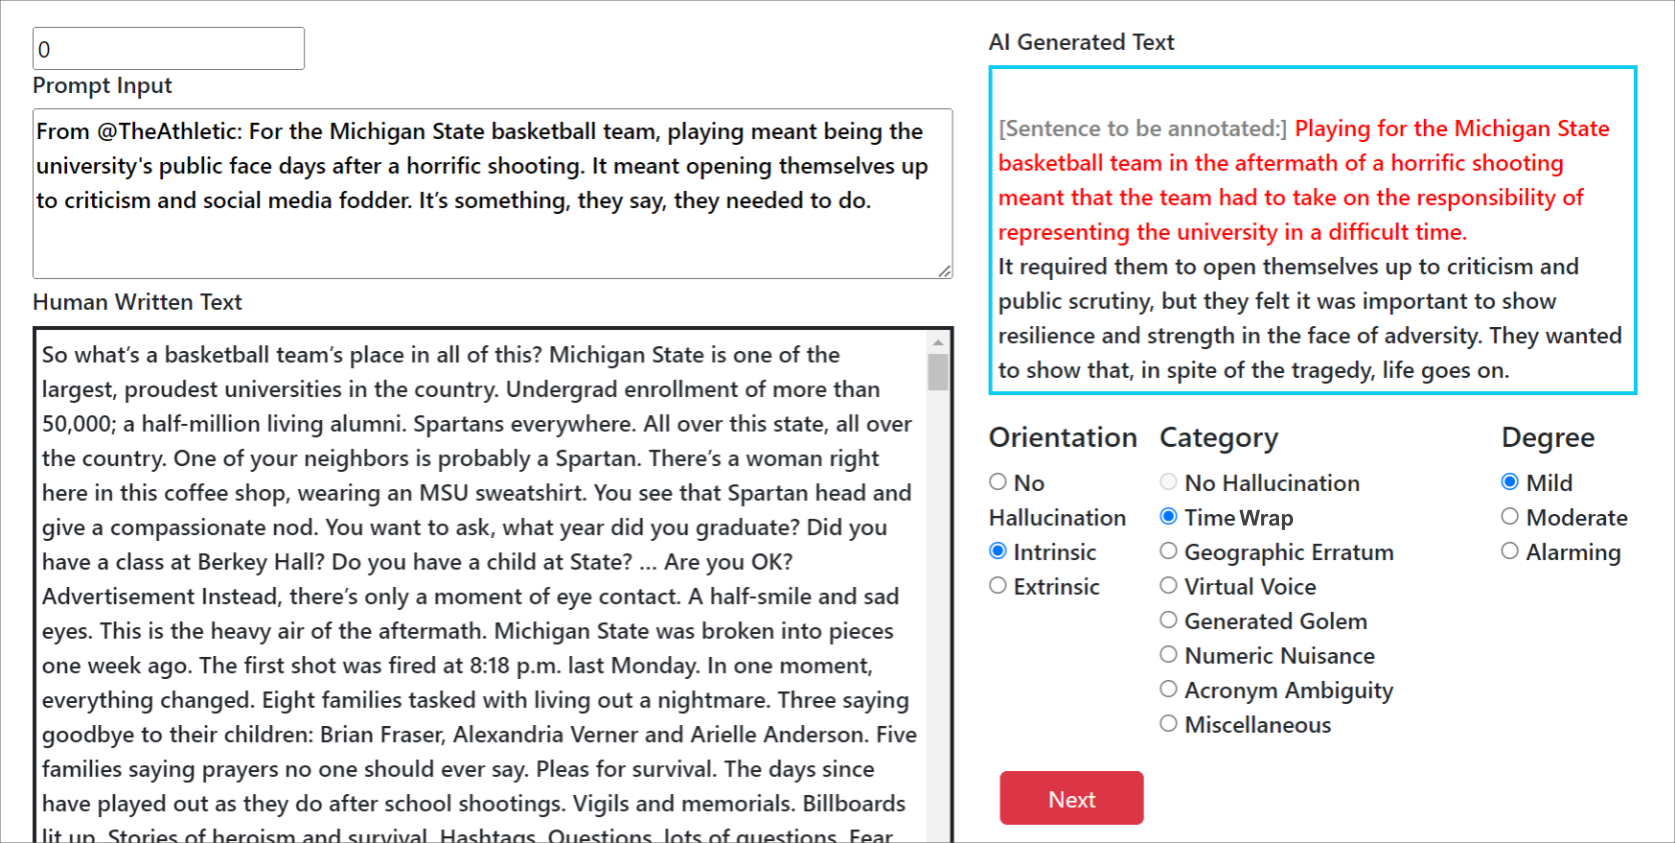
\includegraphics[width=\columnwidth, height=8.8cm]{img/web_img.png}
    \caption{Web interface used to annotate the HILT dataset using  Amazon Mechanical Turk.}
    \vspace{-3mm}
    \label{fig:web}
%\end{wrapfigure}
\end{figure*}

In order to facilitate the annotation process for the annotators, it is crucial to provide them with a user-friendly interface that enables easy navigation. \cref{fig:web} shows our annotation web interface used to construct the HILT dataset. The interface is designed to offer a comprehensive view to the annotator. For instance, at the top of the interface, the actual prompt used for generating the text snippet is displayed. Directly below the prompt, the complete AI-generated text is shown. On the right-hand side, the sentence breakup is presented, with the currently selected sentence highlighted in red. Below the sentence breakup, all the relevant categories are displayed as radio buttons, allowing the annotators to easily annotate each category. This interface aims to enhance the efficiency and effectiveness of the annotation process. We have gone through a few rounds of iterations before finalizing the current version of the web interface. 


\subsection{Selecting quality annotators on AMT}
% Please add the following required packages to your document preamble:
% \usepackage{booktabs}
% \usepackage{graphicx}
% \vspace{-1mm}
\begin{wraptable}{R}{10cm}
\centering
\resizebox{0.6\columnwidth}{!}{%
\begin{tabular}{@{}ll|lc|ll@{}}
\toprule
\multicolumn{1}{c}{\textbf{Orientation}} &
  \multicolumn{1}{c|}{\textbf{Annotation}} &
  \multicolumn{1}{c}{\textbf{Category}} &
  \textbf{Annotation} &
  \multicolumn{1}{c}{\textbf{Degree}} &
  \multicolumn{1}{c}{\textbf{Annotation}} \\ \midrule
No Hallucination        & \multicolumn{1}{c|}{0} & No Hallucination   & 0 & Mild     & \multicolumn{1}{c}{0} \\
Intrinsic Hallucination & \multicolumn{1}{c|}{1} &     Time Wrap    & 1 & Moderate & \multicolumn{1}{c}{1} \\
Extrinsic Hallucination & \multicolumn{1}{c|}{2} & Geographic Erratum & 2 & Alarming & \multicolumn{1}{c}{2} \\
                        &                        & Virtual Voice      & 3 &          &                       \\
                        &                        & Generated Golem    & 4 &          &                       \\
                        &                        & Numeric Nuisance   & 5 &          &                       \\
                        &                        & Acronym Ambiguity  & 6 &          &                       \\
                        &                        & Miscellaneous      & 7 &          &                       \\ \bottomrule
\end{tabular}%
}
\caption{Annotations for 
\includegraphics[height=0.25cm,width=1cm]{img/hilt.png}: Orientation, Category, and Degree. We follow a three-level annotation process where we first determine whether there is a hallucination or not, and if yes, then what orientation. We assign labels 0, 1, and 2 for ``no'', ``intrinsic'', and ``extrinsic'' hallucination. Next, we determine the category of hallucination and label them ranging from 0 through 7, where 7 could be a miscellaneous case where the hallucination does not belong to any category. Finally, the degrees are labeled with 0, 1, and 2.}
\vspace{2mm}
\label{tab:annotations}
\end{wraptable}
It is widely acknowledged that platforms like AMT can be noisy, making the selection of high-quality annotators a critical step in ensuring accurate annotations. The in-house annotation of 2,000 data points played a significant role in achieving this goal. To identify reliable annotators, we initiated a pilot task and only selected those with an accuracy rate of over 90\% based on our in-house annotated dataset.

Another crucial consideration when annotating data on crowdsourcing platforms is the compensation offered to annotators. While offering too little may deter interest, excessively high wages may attract undesirable spammers. Achieving the ideal balance required several rounds of iteration to determine an appropriate compensation scheme.

By carefully addressing factors such as selecting qualified annotators and establishing suitable compensation rates, we improved the quality of annotations obtained from crowdsourcing platforms.



\subsection{Inter-Annotator Agreement}
We report Fleiss's kappa ($\kappa$) \cite{Wikipedia-Kappa} and Krippendorff's alpha ($\alpha$) \cite{Wikipedia-Alpha} scores (see \cref{tab:inter-annot-nyt,tab:inter-annot-pol}) to access the reliability of agreement between the three annotators\footnote{Three graduate students}. We compute agreement on 10\% of total annotated entities and obtain  substantial to almost perfect agreement in all three annotation types in both datasets, namely NYT and Politifact. We have obtained nearly or more than 80\% agreement in the case of \texttt{orientation} and \texttt{category}. The agreement on \texttt{degree} exhibits slight variation, as it relies on the subjective assessment of the percentage of hallucination in the sentence. This interpretation of percentage tends to differ among individuals. We report both Fleiss's kappa and Krippendorff's alpha score because Fleiss's kappa is a statistical measure that allows us to find agreement among multiple annotators and Krippendorff's alpha is a statistical measure that allows us to handle various types of data like nominal (\texttt{orientation} and \texttt{category}) and ordinal (\texttt{degree}). \\

\noindent
\begin{minipage}[c]{0.5\textwidth}
%\begin{table}[!htp]
\centering
\scriptsize
\resizebox{0.95\columnwidth}{!}{%
\begin{tabular}{lcc}\toprule
&\textbf{Fleiss's kappa} & \textbf{Krippendorff's alpha} \\\midrule
\textbf{Orientation} & 0.7911 & 0.8146 \\
\textbf{Category} & 0.7846 & 0.8499 \\
\textbf{Degree} & 0.7473 & 0.7274 \\
\bottomrule
\end{tabular}%
}
\captionof{table}{Inter-annotator scores for NYT dataset.}
\label{tab:inter-annot-nyt}
%\end{table}
\end{minipage}
\begin{minipage}[c]{0.5\textwidth}
%\begin{table}[!htp]
%\centering
\scriptsize
\resizebox{0.95\columnwidth}{!}{%
\begin{tabular}{lcc}\toprule
&\textbf{Fleiss's kappa} & \textbf{Krippendorff's alpha} \\\midrule
\textbf{Orientation} & 0.7587 & 0.8436 \\
\textbf{Category} & 0.8755 & 0.9328 \\
\textbf{Degree} & 0.6182 & 0.5455 \\
\bottomrule
\end{tabular}%
}
\captionof{table}{Inter-annotator scores for Politifact dataset.}
\label{tab:inter-annot-pol}
\end{minipage}
%\end{table}


% Under Step 3, we identify the degree of hallucination as low, moderate, or high. If the sentence is delivering completely delusional information, then we identify it as a high degree of hallucination. If the sentence is delivering partially delusional information, then we identify it as a moderate degree of hallucination. Similarly, for a very less amount of delusional information, we identify it as a low degree of hallucination. After identification, our annotations are as follows,


\section{Details on chosen LLMs}
\subsection{Criteria for choosing LLMs}\label{apdx:llm-select}

Beyond the primary criteria for choosing performant LLMs, our selection was meant to cover a wide gamut of LLMs that utilize a repertoire of recent techniques under the hood that have enabled their exceptional capabilities, namely: 

\vspace{-2mm}
\begin{itemize}
[leftmargin=10mm]
\setlength\itemsep{0em}
\item FlashAttention \cite{dao2022flashattention} for memory-efficient exact attention.
\item Multi-Query Attention \cite{shazeer2019fast} for memory bandwidth efficiency.
\item SwiGLU \cite{shazeer2020glu} as the activation function instead of ReLU \cite{agarap2019deep}.
\item ALiBi \cite{DBLP:conf/iclr/PressSL22} for larger context width.
\item RMSNorm \cite{zhang2019root} for per-normalization.
\item RoPE \cite{su2022roformer} to improve the expressivity of positional embeddings, etc.
\end{itemize}


\subsection{Details on Large Language Models}
Model details are given in \cref{tab:hf-links}. We use HuggingFace \cite{wolf2020huggingfaces} and OpenAI for implementing the large language models to generate the dataset.


\begin{comment}
\begin{itemize} %enumerate}

  \item \textbf{MPT \cite{wang2023multitask}} is a part of the family of MosaicPretrainedTransformer(MPT) models, which use a modified transformer architecture optimized for efficient training and inference.
  
  \item \textbf{StableLM \cite{liu2023your}} The Alpha version of the model is available in 3 billion and 7 billion parameters.

  \item \textbf{Dolly \cite{dolly}} is an instruction-following large language model trained on the Databricks machine learning platform.
  
  \item \textbf{Vicuna \cite{vicuna2023}} is created by fine-tuning a LLaMA base model using approximately 70K user-shared conversations gathered from ShareGPT.com
  
  \item \textbf{GPT4 \cite{openai2023gpt4}} was released by OpenAI in 2023. It is a large multimodal model that shows human-level performance on various professional and academic benchmarks.
  
  \item \textbf{Alpaca \cite{alpaca}}  is a language model fine-tuned using supervised learning from a LLaMA 7B model on 52K instruction-following demonstrations.
  
  \item \textbf{LLaMa \cite{touvron2023llama}} is a collection of foundation language models varying from 7B to 65B parameters. It is trained on trillions of tokens. LLaMA-13B outperforms GPT-3 (175B) on most benchmarks.
  
  \item \textbf{GPT3.5 \cite{openaisafety}} is a sub-class of GPT-3 model family. It has 3 variants each with 1.3B, 6B, and 175B parameters.
  
  \item \textbf{BLOOM \cite{scao2022bloom}} is similar to GPT3 (auto-regressive model for next token prediction). However, it has been trained on 46 different languages and 13 programming languages.
  
  \item \textbf{OPT \cite{zhang2022opt}} is a decoder-only pre-trained transformer model ranging from 125M to 175B parameters.  Although the performance of OPT-175B is comparable to GPT-3, it only requires 1/7th the carbon footprint to develop. 

  \item \textbf{T0 \cite{DBLP:conf/iclr/DeleuKFKBLB22}} is trained on a diverse set of tasks and prompts leading to increased robustness to the prompt wording. T0 outperforms or matches GPT-3, which is 16x larger in size and has 100s of billions of parameters.
   
  \item \textbf{GPT3 \cite{brown2020language}} is an autoregressive language model by OpenAI. It is a decoder-only transformer model with a size of 175 billion parameters. 

  \item \textbf{T5 \cite{raffel2020exploring}} is an encoder-decoder model pre-trained on a multi-task combination of unsupervised and supervised tasks Each task is converted into a text-to-text format. 
  
  \item \textbf{XLNet \cite{yang2019xlnet}} is a generalized autoregressive pretraining model that (1) enables learning bidirectional contexts by maximizing the expected likelihood over all permutations of the factorization order and (2) overcomes the limitations of BERT because of its own autoregressive formulation. 

  \item \textbf{GPT2 \cite{radford2019language}} is a large transformer-based language model with 1.5 billion parameters. It is trained on a WebText dataset consisting of 8 million web pages. 
\end{itemize}  %enumerate}
\end{comment}


\begin{table}[!htp]\centering
\scriptsize
%\resizebox{\columnwidth}{!}{%
\begin{tabular}{p{1cm}|p{1.1cm}|p{3cm}|p{8.9cm}}\toprule
\textbf{LLMs} &\textbf{Parameter size} &\textbf{LLM used in this paper}  &\textbf{Details}\\\midrule
GPT-3 &175B & \href{https://platform.openai.com/docs/models/gpt-3}{gpt3} &  \textbf{GPT-3 \cite{brown2020language}} is an autoregressive language model by OpenAI. It is a decoder-only transformer model with a size of 175 billion parameters. \\ \midrule
StableLM &7B &\href{https://huggingface.co/stabilityai/stablelm-base-alpha-7b}{stablelm-base-alpha-7b} & \textbf{StableLM \cite{liu2023your}} The Alpha version of the model is available in 3 billion and 7 billion parameters.\\ \midrule
GPT-2 &1.5B &\href{https://huggingface.co/gpt2}{gpt2} & \textbf{GPT-2 \cite{radford2019language}} is a large transformer-based language model with 1.5 billion parameters. It is trained on a WebText dataset consisting of 8 million web pages. \\ \midrule
Vicuna &13B &\href{https://huggingface.co/eachadea/vicuna-13b-1.1}{eachadea//vicuna-13b-1.1} & \textbf{Vicuna \cite{vicuna2023}} is created by fine-tuning a LLaMA base model using approximately 70K user-shared conversations gathered from ShareGPT.com\\ \midrule
MPT &7B & \href{https://huggingface.co/mosaicml/mpt-7b}{mosaicml/mpt-7b} & \textbf{MPT \cite{wang2023multitask}} is a part of the family of MosaicPretrainedTransformer(MPT) models, which use a modified transformer architecture optimized for efficient training and inference.\\ \midrule
LLaMA &65B &\href{https://huggingface.co/decapoda-research/llama-65b-hf}{decapoda-research/llama-65b-hf} & \textbf{LLaMa \cite{touvron2023llama}} is a collection of foundation language models varying from 7B to 65B parameters. It is trained on trillions of tokens. LLaMA-65B outperforms GPT-3 (175B) on most benchmarks.\\  \midrule
GPT-3.5 &175B & \href{https://platform.openai.com/docs/models/gpt-3-5}{gpt3.5 (text-davinci-003)} &  \textbf{GPT-3.5 \cite{openaisafety}} is a sub-class of GPT-3 model family. It has 3 variants each with 1.3B, 6B, and 175B parameters.\\  \midrule
Dolly &12B &\href{https://huggingface.co/databricks/dolly-v2-12b}{dolly-v2-12b} & \textbf{Dolly \cite{dolly}} is an instruction-following large language model trained on the Databricks machine learning platform.\\  \midrule
OPT &175B &\href{https://github.com/facebookresearch/metaseq/tree/main/projects/OPT}{opt-175B} & \textbf{OPT \cite{zhang2022opt}} is a decoder-only pre-trained transformer model ranging from 125M to 175B parameters.  Although the performance of OPT-175B is comparable to GPT-3, it only requires 1/7th the carbon footprint to develop.\\ \midrule
GPT-4 &170T & \href{https://openai.com/research/gpt-4}{gpt4} & \textbf{GPT-4 \cite{openai2023gpt4}} was released by OpenAI in 2023. It is a large multimodal model that shows human-level performance on various professional and academic benchmarks. \\  \midrule
Alpaca &7B &\href{https://huggingface.co/chainyo/alpaca-lora-7b}{chainyo/alpaca-lora-7b} & \textbf{Alpaca \cite{alpaca}}  is a language model fine-tuned using supervised learning from a LLaMA 7B model on 52K instruction-following demonstrations.\\ \midrule
BLOOM &176B &\href{https://huggingface.co/bigscience/bloom}{bigscience/bloom} & \textbf{BLOOM \cite{scao2022bloom}} is similar to GPT-3 (auto-regressive model for next token prediction). However, it has been trained on 46 different languages and 13 programming languages.\\ \midrule
T0 &11B &\href{https://huggingface.co/bigscience/T0}{bigscience/T0} & \textbf{T0 \cite{DBLP:conf/iclr/DeleuKFKBLB22}} is trained on a diverse set of tasks and prompts leading to increased robustness to the prompt wording. T0 outperforms or matches GPT-3, which is 16x larger in size and has 100s of billions of parameters.\\ \midrule
XLNet &340M &\href{https://huggingface.co/xlnet-large-cased}{xlnet-large-cased} & \textbf{XLNet \cite{yang2019xlnet}} is a generalized autoregressive pretraining model that (1) enables learning bidirectional contexts by maximizing the expected likelihood over all permutations of the factorization order and (2) overcomes the limitations of BERT because of its own autoregressive formulation. \\ \midrule
T5 &11B &\href{https://huggingface.co/t5-11b}{t5-11b} & \textbf{T5 \cite{raffel2020exploring}} is an encoder-decoder model pre-trained on a multi-task combination of unsupervised and supervised tasks Each task is converted into a text-to-text format. \\ 


\bottomrule
\end{tabular}

\caption{HuggingFace and OpenAI links for all LLMs.}
\label{tab:hf-links}
\end{table}


\section{
\includegraphics[width=0.9cm]{img/hilt.png} - Prompt sources}
We used two datasets to curate HILT: (i) New York Times Tweets \cite{nyt} for factually correct and (ii) Politifact dataset \cite{Politifact} for factually incorrect prompts.


\section{What is a high entropy vs. low entropy word?}
\label{sec:entropy}
\vspace{-2mm}
%\begin{wrapfigure}{L}{13.5cm}
\begin{figure*}[!ht]  
\centering
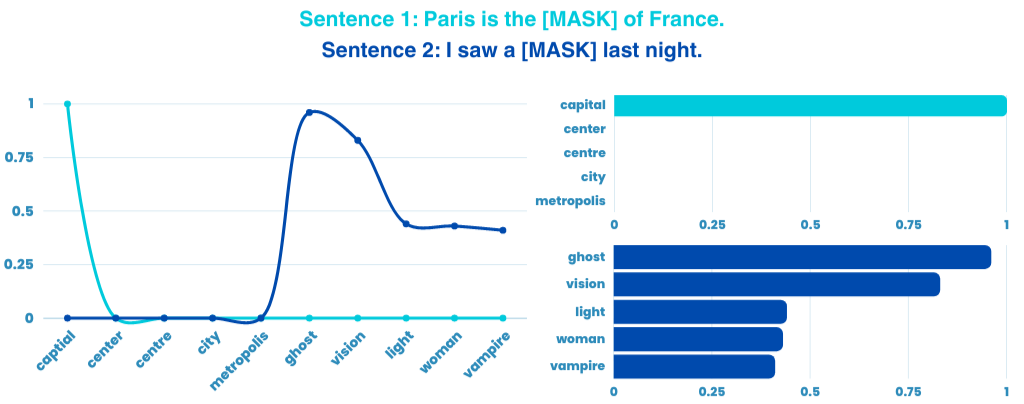
\includegraphics[height=6.5cm,width=\columnwidth]{img/entropy-cropped.png}
    \caption{High entropy word vs. low entropy word - a side-by-side illustration.}
    \vspace{-3mm}
    \label{fig:entropy}
\end{figure*}
%\end{wrapfigure}

In the context of language modeling, a high entropy word refers to a word or token that has a high level of uncertainty or unpredictability in its occurrence. In other words, it is a word that is relatively rare or has a low probability of appearing in a given context. Entropy is often used to quantify the level of unpredictability associated with generating specific words or tokens. When a language model encounters a high entropy word, it means that the model has greater difficulty in accurately predicting or generating that word based on the context or preceding words. High entropy words are often less frequent in the training data or have complex patterns of occurrence. For example, in a language model trained on news articles, words like ``pneumonoultramicroscopicsilicovolcanoconiosis'' (a technical term for a lung disease) would likely have high entropy, as they are infrequent and occur in specific contexts.

On the other hand, a low entropy word refers to a word or token that has a relatively high predictability or a limited range of potential next words given the context. In other words, it is a word that occurs frequently and is highly expected in a specific context. When a language model encounters a low entropy word, it means that the model has a higher confidence or accuracy in predicting or generating that word based on the context or preceding words. For example, in a language model trained on English text, common words like ``the,'' ``and,'' or ``is'' have low entropy because they occur frequently and are highly predictable in many contexts. These words tend to have a limited set of likely next words based on the preceding context. \cref{fig:entropy} illustrates an example of the entropy distribution over the set of words in an input sentence. In sentence 1, \texttt{[MASK]} token has low entropy since \texttt{capital} is the highest probable word in that sentence.  However, \texttt{[MASK]} token in sentence 2 has high entropy since it is quite uncertain as to what the masked token could be. The probability distributions for this illustration are created using the HuggingFace Inference API \cite{HuggingFaceInfAPI}.


%\acil{@Vipula, add the source of the figure (which HuggingFace spaces demo is this?). Also, can we add two more examples here so we can call it a "case study"?}



\begin{comment}
\section{HVI vs. LLMs size for different LLMs: An insight from 
\includegraphics[width=1cm]{img/hilt.png}}
\label{app:llm-size}
\vspace{-2mm}
\begin{wrapfigure}{R}{11cm}
    \centering
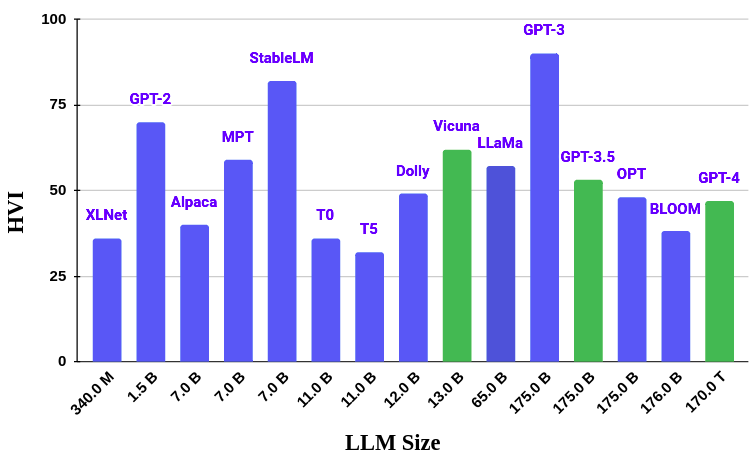
\includegraphics[width=0.7\columnwidth]{img/chart.png}
    \caption{\emph{HVI} vs. \emph{LLM size} for different LLMs.}
    \vspace{-3mm}
    \label{fig:llm-size}
\end{wrapfigure}
There is a general observation that larger language models (LLMs) may exhibit a higher tendency towards generating hallucinations or producing outputs that deviate from factual or coherent information. However, it's important to note that the relationship between LLM size and hallucination is not necessarily a direct correlation, but rather a consideration based on certain factors such as (a) training data quality, (b) lack of explicit training on facts, and (c) overconfidence in generated responses. A noteworthy pattern that emerges is that LLMs without RLHF (Reinforcement Learning from Human Feedback) \cite{DBLP:journals/corr/abs-1909-08593} tend to exhibit a higher tendency for hallucination. Although we did not extensively evaluate this phenomenon, we have a keen interest in investigating it further in the near future.
%\textcolor{red}{Our empirical findings show that the....finish this sentence after empirical results?}
\cref{fig:llm-size} shows how HVI and LLM size are correlated and hence, larger LLM tends to hallucinate more.
\end{comment}


\begin{comment}
\begin{table*}[!ht]%[H]
\resizebox{\textwidth}{!}{%
\begin{tabular}{p{0.05\textwidth} | p{0.95\textwidth}} %{ll}
\toprule
{\footnotesize Prompt}            
& 
\begin{footnotesize}
USA and UK are collaborating to tackle Biohazards to address Climate Control  
\end{footnotesize}
\\ \hline
\rotatebox[origin=r]{90}{\parbox[c]{2.5cm}{\centering {\footnotesize AI-generated text}}}
& 
\begin{footnotesize}
In a significant development, the United States of America (USA) and the United Kingdom (UK) have announced a collaborative effort to address the critical issue of biohazards in the realm of climate control. Through this partnership, the USA and UK aim to enhance their preparedness and response mechanisms to effectively combat biohazards resulting from climate change. By sharing scientific knowledge, technological advancements, and best practices. \hlpink{USA President George W. Bush and UK Prime Minister Boris Johnson}, along with a delegation of experts, are convening today in London to discuss and elaborate on the critical issue of biohazards in climate control.
\end{footnotesize}
\\ \hline
{\footnotesize Fact}
& 
\begin{footnotesize}
\hlgreen{George W. Bush holds the presidency during 2001-2009 and Boris Johnson was in the PM position during 2019-2022. Not possible to meet each other as president and as PM.} 
\end{footnotesize}
\\ 
\toprule
{\footnotesize Prompt}
&  
\begin{footnotesize}
Scientists in the US have announced the discovery of water on Pluto  
\end{footnotesize}
\\ \hline
\rotatebox[origin=r]{90}{\parbox[c]{2.5cm}{\centering {\footnotesize AI-generated text}}}
& 
\begin{footnotesize}
\hlpink{Pluto is the planet that has long been considered a desolate wasteland. The presence of water on Pluto is a major breakthrough for our understanding of the Solar System and could lead to further discoveries about other planets. The team, led by Professor Alan Stern from Brown University, used data from the New Horizons spacecraft to uncover evidence of water ice on the surface of Pluto. The ice appears to be concentrated in certain areas, suggesting that it may be possible to find liquid water there. This discovery raises many questions about how life could exist on Pluto and whether or not it might be possible to explore it further. Professor Stern said: ``This is an exciting finding because we thought.} 
\end{footnotesize}
\\ \hline
{\footnotesize Fact}
& 
\begin{footnotesize}
\hlgreen{There is no such discovery! Professor Alan Stern from Brown University is a real person, who was the principal investigator of the New Horizons mission to Pluto, but never said this.} 
\end{footnotesize}
\\ \bottomrule
\end{tabular}%
}
\caption{Hallucination examples with NYT tweets as prompts. \adt{need a detailed caption}}
\label{tab:hallucination_ex}
\end{table*}
\end{comment}



\begin{comment}
\subsection{Intrinsic Hallucination}

\textbf{AI generated text 1070:} ``Dr. Ward Stone began his career as a wildlife pathologist in New York State in the 1970s. He quickly became known for his maverick approach to his job, which often meant going beyond his mandate to investigate the effects of toxic chemicals on both wildlife and people. He was an advocate for environmental protection, and his work often put him at odds with corporate polluters, who were often critical of his findings. Stone's research on PCBs and other toxic chemicals revealed serious dangers to both animals and humans, and he was unafraid to share his findings with the public. His work led to some significant breakthroughs, including the discovery of the first link between PCBs, cancer, and reproductive problems in people. He was also vocal in his criticism of the state and federal governments for not doing enough to protect the environment. Stone received a number of awards and honors for his work during his career, including the Audubon Medal, the highest honor given by the National Audubon Society. He was also inducted into the New York State Environment Hall of Fame in 2015. \hlpink{Stone passed away in 2019 at the age of 94.} His legacy as an environmental advocate and scientist will continue to be remembered for many years to''

\hlgreen{Dr. Ward had actually died at the age of 84 in 2023.}


\subsection{Extrinsic Hallucination}

\textbf{AI generated text 4:} 

``Walmart said that while it saw strong growth in its online business, higher prices in certain categories, such as food and apparel, led to an overall decline in consumer spending. Walmart also said that rising prices of goods such as fuel, apparel, and food have caused customers to become more price-conscious, and that the current economic environment is creating a ``headwind'' for the company. In response to this economic climate, Walmart is taking steps to make sure customers are getting the best value for their money. Walmart is focusing on offering low prices on everyday items, using a combination of discounts and promotions. The company is also investing in its online and mobile capabilities, to make it easier for customers to shop and save online. Walmart is also investing in its stores, to make sure they are providing the best customer service and shopping experience possible. Walmart is also working to reduce costs in order to maintain its low-price strategy. \hlpink{The company is implementing cost-cutting measures, such as reducing its store-level workforce and increasing automation in its distribution centers. Overall, Walmart is taking steps to ensure that it can remain competitive in a tough economic environment. The company is focusing on offering low prices and investing in its online and''.}

\hlgreen{There is no perfect evidence on whether the company is taking such measures or not.}
\end{comment}




\section{Mitigation Techniques: The specifics}
\label{sec:mitigation_appendix}
In addition to the ~\cref{tab:hallucination_ex} provided in ~\cref{sec:mitigation}, we now present two additional illustrative examples in \cref{tab:hallucination_ex_3} and \cref{tab:hallucination_ex_2} to demonstrate the practical application of two different mitigation techniques.


%Example #2
%\vspace{-8mm}
\begin{table}[htp!]
\centering
\resizebox{0.92\textwidth}{!}{%
\begin{tabular}{p{0.06\textwidth}|p{1.5\textwidth}} \toprule
{\footnotesize \textbf{Prompt}} 
& \begin{Large}
\textit{There are more oil rigs in operation in the United States than the rest of the world combined.}
\end{Large} \\ \hline
\rotatebox[origin=r]{90}{\parbox[c]{2cm}{\centering {\footnotesize \textbf{Hallucinated text}}}}
& 
\begin{Large}
{This is not true. According to the \colorbox{LightBlue}{International Association of Oil and Gas Producers}, as of the start
of \colorbox{LightBlue}{2020}, \colorbox{pink}{there were a total of \colorbox{LightBlue}{4,932} \colorbox{LightBlue}{oil rigs} in operation worldwide}, with the \colorbox{LightBlue}{United States} having
\colorbox{LightBlue}{1,094} of them. This means that the \colorbox{LightBlue}{US} has \colorbox{LightBlue}{22.1\%} of the world’s total \colorbox{LightBlue}{oil rigs} in operation.
}
\end{Large} \\ \hline
\rotatebox[origin=r]{90}{\parbox[c]{2cm}{\centering {\footnotesize \textbf{Mitigated text\\\textcolor{blue}{ENTROPY\textsubscript{BB}}}}}}
& 
\begin{Large}
This is not true. According to the \colorbox{Thistle}{company} as of the start of \colorbox{Thistle}{year} there were a total of \colorbox{Thistle}{number} \colorbox{Thistle}{wells} in operation worldwide with the \colorbox{Thistle}{unknown} having \colorbox{Thistle}{number} of them. This means that the \colorbox{Thistle}{country} has \colorbox{Thistle}{number} of the world’s total \colorbox{Thistle}{wells} in operation.
\end{Large} \\ \hline
\rotatebox[origin=r]{90}{\parbox[c]{2.5cm}{\centering {\footnotesize \textbf{Edit Suggestions\\\textcolor{blue}{FACTUALITY\textsubscript{GB}}}}}}
& 
\begin{Large}
This is not true. \colorbox{PeachPuff}{According to the International Association of Oil and Gas Producers, as of the start of 2020, there} \colorbox{PeachPuff}{were a total of 4,932 oil rigs in operation worldwide, with the United States having 1,094 of them.} This means that the US has 22.1\% of the world’s total oil rigs in operation.
\end{Large}  \\ \bottomrule
\end{tabular}%
}
\vspace{-2mm}
\caption{A hallucination example pre- and post-mitigation. \colorbox{pink}{A} - hallucinated fragments, \colorbox{LightBlue}{B} - high entropy fragments, \colorbox{Thistle}{C} - replaced text, \colorbox{Khaki}{D} - highlighted text for no information found, and \colorbox{PeachPuff}{E} - refuted text fragments by textual entailment.} 
\label{tab:hallucination_ex_3}
\end{table}


\begin{table}[H]
\centering
\resizebox{0.92\textwidth}{!}{%
\begin{tabular}{p{0.06\textwidth}|p{1.5\textwidth}} \toprule
{\footnotesize \textbf{Prompt}} 
& \begin{Large}
\textit{Rescue workers in Turkey are battling exhaustion as the hope of finding more earthquake survivors
dwindles. Remembering those they have saved spurs them to keep searching. A powerful new quake
on Monday complicated their task.
}
\end{Large}
\\ \hline
\rotatebox[origin=r]{90}{\parbox[c]{2cm}{\centering {\footnotesize \textbf{Hallucinated text}}}}
& 
\begin{Large}
{The \colorbox{LightBlue}{7.0} magnitude quake that \colorbox{LightBlue}{rocked} the \colorbox{LightBlue}{Aegean Sea} was \colorbox{LightBlue}{Turkey’s} deadliest in a decade, killing at
least \colorbox{LightBlue}{109} people and injuring more than \colorbox{LightBlue}{1,000}. It \colorbox{LightBlue}{toppled dozens of buildings} in the cities of \colorbox{LightBlue}{Izmir}
and \colorbox{LightBlue}{Mugla} and left \colorbox{LightBlue}{dozens} of people \colorbox{LightBlue}{trapped} beneath the rubble. Rescue crews have worked tirelessly
all week, often in the dark and in \colorbox{LightBlue}{perilous} conditions. At the same time, they have had to cope with
the emotional toll of finding bodies, many of them children, in the debris. \colorbox{pink}{\colorbox{LightBlue}{One} rescuer, \colorbox{LightBlue}{Hasan Cetin}, said he was motivated by the thought of the survivors he helped save. ``The moment} \colorbox{pink}{when a man ora child is pulled out of the ruins, the joy of seeing them come back to life is indescribable.}” Cetin
told The Associated Press “This is why we keep on going.'' The rescuers have been buoyed by the
support of local people, who have donated food, water, and other supplies. Turkey’s \colorbox{LightBlue}{Health} Minister
\colorbox{LightBlue}{Fahrettin Koca} said \colorbox{LightBlue}{Monday} that the rescue efforts would continue until the last victim was found.}
\end{Large}
\\ \hline
\rotatebox[origin=r]{90}{\parbox[c]{2cm}{\centering {\footnotesize \textbf{Mitigated text\\\textcolor{blue}{ENTROPY\textsubscript{BB}}}}}}
& 
\begin{Large}
The \colorbox{Thistle}{high} magnitude quake that \colorbox{Thistle}{shook} the \colorbox{Thistle}{south} was \colorbox{Thistle}{country’s} deadliest in a decade killing at least \colorbox{Thistle}{number} people and injuring more than \colorbox{Thistle}{number}. It \colorbox{Thistle}{affected a lot of buildings} in the cities of \colorbox{Thistle}{unknown} and \colorbox{Thistle}{unknown} and left dozens of people trapped beneath the rubble. Rescue crews have worked tirelessly all week often in the dark and in \colorbox{Thistle}{severe} conditions. At the same time, they have had to cope with the \colorbox{Thistle}{trauma} of finding bodies many of them children in the \colorbox{Thistle}{unknown}. \colorbox{Thistle}{Local} rescuer \colorbox{Thistle}{person} said he was motivated by the thought of the survivors he helped save “The moment when a man or a child is pulled out of the \colorbox{Thistle}{dust} the \colorbox{Thistle}{fear} of seeing them come back to life is indescribable”. \colorbox{Thistle}{Someone} told The \colorbox{Thistle}{media} “This is why we keep on going” The rescuers have been \colorbox{Thistle}{obliged} by the support of local people who have donated food water and other supplies \colorbox{Thistle}{Country's} Health Minister \colorbox{Thistle}{also} said \colorbox{Thistle}{friday} that the rescue efforts would continue until the last victim was found.
\end{Large}
\\ \hline
\rotatebox[origin=r]{90}{\parbox[c]{2.5cm}{\centering {\footnotesize \textbf{Edit Suggestions\\\textcolor{blue}{FACTUALITY\textsubscript{GB}}}}}}
& 
\begin{Large}
The 7.0 magnitude quake that rocked the Aegean Sea was Turkey's deadliest in a decade, killing at
least 109 people and injuring more than 1,000. It toppled dozens of buildings in the cities of Izmir
and Mugla and left dozens of people trapped beneath the rubble. Rescue crews have worked tirelessly
all week, often in the dark and in perilous conditions. At the same time, they have had to cope with
the emotional toll of finding bodies, many of them children, in the debris. \colorbox{Khaki}{One rescuer, Hasan Cetin, said he was motivated by the thought of the survivors he helped save. ``The moment when} \colorbox{Khaki}{a man or a child is pulled out of the ruins, the joy of seeing them come back to life is indescribable.}''. \colorbox{Khaki}{Cetin told The Associated Press “This is why we keep on going.”} The rescuers have been buoyed by the support of local people, who have donated food, water, and other supplies. Turkey’s Health Minister
Fahrettin Koca said Monday that the rescue efforts would continue until the last victim was found.
\end{Large}
\\ \bottomrule
\end{tabular}%
}
\vspace{-2mm}
\caption{A hallucination example pre- and post-mitigation. \colorbox{pink}{A} - hallucinated fragments, \colorbox{LightBlue}{B} - high entropy fragments, \colorbox{Thistle}{C} - replaced text, \colorbox{Khaki}{D} - highlighted text for no information found, and \colorbox{PeachPuff}{E} - refuted text fragments by textual entailment.} 
\label{tab:hallucination_ex_2}
\end{table}






\begin{comment}
\begin{table}[htp!]
\resizebox{0.98\textwidth}{!}{%
\begin{tabular}{p{0.06\textwidth} | p{1.5\textwidth}} %{ll}
\centering
\toprule
{\footnotesize \textbf{Prompt}} 
& 
\toprule
\begin{Large}
\textit{Barack Obama has never even worked in business.}
\end{Large}
\\ \hline
\rotatebox[origin=r]{90}{\parbox[c]{2cm}{\centering {\footnotesize \textbf{Hallucinated text}}}}
& 
\begin{Large}
{It is true that former \colorbox{LightBlue}{President Barack Obama} did not have significant experience working in the
private sector before entering politics. However, \colorbox{pink}{it is also true that he and his childhood friend
\colorbox{LightBlue}{Mike} formed a small \colorbox{LightBlue}{business} venture called} \colorbox{pink}{Business \colorbox{LightBlue}{International Corporation (BIC)} in \colorbox{LightBlue}{1985}}. \colorbox{LightBlue}{BIC}
provided research and consulting services to American companies seeking to do business overseas.
While \colorbox{LightBlue}{BIC} was not a large-scale operation and ultimately closed down after a few years due to
financial difficulties, it does represent \colorbox{LightBlue}{one} example of \colorbox{LightBlue}{Obama}’s early entrepreneurial activity outside
of politics.
}
\end{Large}
\\ \hline
\rotatebox[origin=r]{90}{\parbox[c]{2cm}{\centering {\footnotesize \textbf{Mitigated text\\\textcolor{blue}{ENTROPY\textsubscript{BB}}}}}}
& 
\begin{Large}
It is true that former President Barack Obama did not have significant experience working in the private sector before entering politics However it is also true that he and his childhood friend \colorbox{Thistle}{clinton} formed a small business venture called \colorbox{Thistle}{obama consulting or bic} in which BIC provided research and consulting services to American companies seeking to do business overseas While BIC was not a large-scale operation and ultimately closed down after a few years due to financial difficulties it does represent one example of Obama’s early entrepreneurial activity outside of politics.
\end{Large}
\\ \hline
\rotatebox[origin=r]{90}{\parbox[c]{2.5cm}{\centering {\footnotesize \textbf{Edit Suggestions\\\textcolor{blue}{FACTUALITY\textsubscript{GB}}}}}}
& 
\begin{Large}
It is true that former President Barack Obama did not have significant experience working in the
private sector before entering politics. However, \colorbox{PeachPuff}{it is also true that he and his childhood friend
Mike formed a small business venture called} \colorbox{PeachPuff}{Business International Corporation (BIC) in 1985.} BIC
provided research and consulting services to American companies seeking to do business overseas.
While BIC was not a large-scale operation and ultimately closed down after a few years due to
financial difficulties, it does represent one example of Obama’s early entrepreneurial activity outside
of politics.
\end{Large}
\\ \bottomrule
\end{tabular}%
}
\vspace{-2mm}
\caption{A hallucination example pre- and post-mitigation. \colorbox{pink}{A} - hallucinated fragments, \colorbox{LightBlue}{B} - high entropy fragments, \colorbox{Thistle}{C} - replaced text, \colorbox{Khaki}{D} - highlighted text for no information found, and \colorbox{PeachPuff}{E} - refuted text fragments by textual entailment.} 
\label{tab:hallucination_ex_3}
%\acil{I recommend replacing this example with an example that has a factual hallucination. Reviewers may argue that the impact of replacing the detected HE words is inconsequential -- it does not significantly change the perception of the story.}
\end{table}
\end{comment}

%\newpage


\subsection{ENTROPY\textsubscript{BB}}
\label{app:bb}

Building upon \cref{sec:mitigation}, \cref{tab:gpt3,tab:StableLM,tab:gpt2,tab:vicuna,tab:mpt,tab:llama,tab:gpt35,tab:dolly,tab:opt,tab:gpt4,tab:alpaca,tab:bloom,tab:t0,tab:xlnet,tab:t5} illustrate the examples of the nuanced categorization of hallucination proposed in the paper.

\begin{comment}
\begin{table}[!htp]
\centering
\scriptsize
\resizebox{\columnwidth}{!}{%
\begin{tabular}{lcccc}\toprule
\textbf{} &\textbf{\texttt{albert-large-v2}} &\textbf{\texttt{bert-base-uncased}} &\textbf{\texttt{distilroberta-base}} &\textbf{\texttt{xlm-roberta-large}} \\\midrule
\textbf{\texttt{albert-large-v2}} &\cellcolor[HTML]{93c47d}6.80 &\cellcolor[HTML]{ffd966}5.40 &\cellcolor[HTML]{ffd966}5.40 &\cellcolor[HTML]{ffd966}5.10 \\
\textbf{\texttt{bert-base-uncased}} &\cellcolor[HTML]{f6b26b}2.70 &\cellcolor[HTML]{f6b26b}2.60 &\cellcolor[HTML]{f6b26b}2.60 &\cellcolor[HTML]{f6b26b}2.50 \\
\textbf{\texttt{distilroberta-base}} &\cellcolor[HTML]{ffd966}4.90 &\cellcolor[HTML]{ffd966}4.40 &\cellcolor[HTML]{ffd966}5.10 &\cellcolor[HTML]{f6b26b}3.30 \\
\textbf{\texttt{xlm-roberta-large}} &\cellcolor[HTML]{f6b26b}2.80 &\cellcolor[HTML]{f6b26b}2.50 &\cellcolor[HTML]{f6b26b}2.70 &\cellcolor[HTML]{f6b26b}2.60 \\
\bottomrule
\end{tabular}%
}
\caption{The row represents the LLM used for detecting high entropy words from StableLM's output, while the column represents the LLM for replacing those words.}
\label{tab:stablelm}
\end{table}
\end{comment}

%\vspace{-4mm}

%GPT-3
\begin{comment}{table}[!htp]\centering
\scriptsize
\resizebox{\columnwidth}{!}{%
\begin{tabular}{lrrrrr}\toprule
\textbf{} &\textbf{\texttt{albert-large-v2}} &\textbf{\texttt{bert-base-uncased}} &\textbf{\texttt{distilroberta-base}} &\textbf{\texttt{xlm-roberta-large}} \\\midrule
\textbf{\texttt{albert-large-v2}} &\cellcolor[HTML]{93c47d}6.72 &\cellcolor[HTML]{f6b26b}3.26 &\cellcolor[HTML]{76a5af}8.66 &\cellcolor[HTML]{93c47d}6.40 \\
\textbf{\texttt{bert-base-uncased}} &\cellcolor[HTML]{ffd966}5.70 &\cellcolor[HTML]{93c47d}7.56 &\cellcolor[HTML]{93c47d}7.98 &\cellcolor[HTML]{93c47d}7.22 \\
\textbf{\texttt{distilroberta-base}} &\cellcolor[HTML]{f6b26b}2.02 &\cellcolor[HTML]{93c47d}7.31 &\cellcolor[HTML]{ffd966}4.55 &\cellcolor[HTML]{76a5af}8.95 \\
\fontfamily{cmtt}\selectfont \textbf{xlm-roberta-large} &\cellcolor[HTML]{f6b26b}2.26 &\cellcolor[HTML]{e06666}2.28 &\cellcolor[HTML]{e06666}1.70 &\cellcolor[HTML]{ffd966}4.78 \\
\bottomrule
\end{tabular}%
}
\caption{GPT-3}
\label{tab:gpt3}
\end{comment}
%\vspace{-4mm}

%GPT-3(new)

\begin{table}[!htp]\centering
\scriptsize
\resizebox{\columnwidth}{!}{%
\begin{tabular}{lrrrrr}\toprule
\textbf{} &\textbf{\texttt{albert-large-v2}} &\textbf{\texttt{bert-base-uncased}} &\textbf{\texttt{distilroberta-base}} &\textbf{\texttt{xlm-roberta-large}} \\\midrule
\textbf{\texttt{albert-large-v2}} &\cellcolor[HTML]{93c47d}6.72 &\cellcolor[HTML]{f6b26b}3.26 &\cellcolor[HTML]{76a5af}\textbf{10.66} &\cellcolor[HTML]{93c47d}6.40 \\
\textbf{\texttt{bert-base-uncased}} &\cellcolor[HTML]{ffd966}4.70 &\cellcolor[HTML]{93c47d}7.56 &\cellcolor[HTML]{93c47d}7.98 &\cellcolor[HTML]{93c47d}7.22 \\
\textbf{\texttt{distilroberta-base}} &\cellcolor[HTML]{f6b26b}2.02 &\cellcolor[HTML]{93c47d}7.31 &\cellcolor[HTML]{ffd966}4.55 &\cellcolor[HTML]{76a5af}9.95 \\
\textbf{\texttt{xlm-roberta-large}} &\cellcolor[HTML]{f6b26b}2.26 &\cellcolor[HTML]{93c47d}6.28 &\cellcolor[HTML]{e06666}1.70 &\cellcolor[HTML]{ffd966}4.78 \\
\bottomrule
\end{tabular}%
}
\caption{Overall drops in hallucination by 16 combinations of 4 LLMs with the rows having the LLMs which detected the high entropy words and the corresponding columns with the LLMs which replaced those words generated by \textbf{GPT-3}. \textbf{10.66} is the maximum drop in overall hallucination detected with \textbf{\texttt{albert-large-v2}} and replaced with \textbf{\texttt{distilroberta-base}}.}
\label{tab:gpt3}
\end{table}

%StableLM
\begin{comment}{table}[!htp]
\centering
\scriptsize
\resizebox{\columnwidth}{!}{%
\begin{tabular}{lcccc}\toprule
\textbf{} &\textbf{\texttt{albert-large-v2}} &\textbf{\texttt{bert-base-uncased}} &\textbf{\texttt{distilroberta-base}} &\textbf{\texttt{xlm-roberta-large}} \\\midrule
\textbf{\texttt{albert-large-v2}} &\cellcolor[HTML]{93c47d}6.80 &\cellcolor[HTML]{ffd966}5.40 &\cellcolor[HTML]{ffd966}5.40 &\cellcolor[HTML]{ffd966}5.10 \\
\textbf{\texttt{bert-base-uncased}} &\cellcolor[HTML]{f6b26b}2.70 &\cellcolor[HTML]{f6b26b}2.60 &\cellcolor[HTML]{f6b26b}2.60 &\cellcolor[HTML]{f6b26b}2.50 \\
\textbf{\texttt{distilroberta-base}} &\cellcolor[HTML]{ffd966}4.90 &\cellcolor[HTML]{ffd966}4.40 &\cellcolor[HTML]{ffd966}5.10 &\cellcolor[HTML]{f6b26b}3.30 \\
\textbf{\texttt{xlm-roberta-large}} &\cellcolor[HTML]{f6b26b}2.80 &\cellcolor[HTML]{f6b26b}2.50 &\cellcolor[HTML]{f6b26b}2.70 &\cellcolor[HTML]{f6b26b}2.60 \\
\bottomrule
\end{tabular}%
}
\caption{StableLM}
\label{tab:StableLM}
\end{comment}
%\vspace{-4mm}


%StableLM(new)
\begin{table}[!htp]\centering
\scriptsize
\resizebox{\columnwidth}{!}{%
\begin{tabular}{lrrrrr}\toprule
\textbf{} &\textbf{\texttt{albert-large-v2}} &\textbf{\texttt{bert-base-uncased}} &\textbf{\texttt{distilroberta-base}} &\textbf{\texttt{xlm-roberta-large}} \\\midrule
\textbf{\texttt{albert-large-v2}} &\cellcolor[HTML]{93c47d}6.80 &\cellcolor[HTML]{ffd966}5.40 &\cellcolor[HTML]{76a5af}\textbf{8.40} &\cellcolor[HTML]{ffd966}5.10 \\
\textbf{\texttt{bert-base-uncased}} &\cellcolor[HTML]{f6b26b}2.70 &\cellcolor[HTML]{f6b26b}2.60 &\cellcolor[HTML]{f6b26b}2.60 &\cellcolor[HTML]{f6b26b}2.50 \\
\textbf{\texttt{distilroberta-base}} &\cellcolor[HTML]{ffd966}4.90 &\cellcolor[HTML]{ffd966}4.40 &\cellcolor[HTML]{ffd966}5.10 &\cellcolor[HTML]{f6b26b}3.30 \\
\textbf{\texttt{xlm-roberta-large}} &\cellcolor[HTML]{f6b26b}2.80 &\cellcolor[HTML]{f6b26b}2.50 &\cellcolor[HTML]{f6b26b}2.70 &\cellcolor[HTML]{f6b26b}2.60 \\
\bottomrule
\end{tabular}%
}
\caption{Overall drops in hallucination by 16 combinations of 4 LLMs with the rows having the LLMs which detected the high entropy words and the corresponding columns with the LLMs which replaced those words generated by \textbf{StableLM}. \textbf{8.40} is the maximum drop in overall hallucination detected with \textbf{\texttt{albert-large-v2}} and replaced with \textbf{\texttt{distilroberta-base}}.}
\label{tab:StableLM}
\end{table}

%GPT-2
\begin{comment}{table}[!htp]\centering
\scriptsize
\resizebox{\columnwidth}{!}{%
\begin{tabular}{lrrrrr}\toprule
\textbf{} &\textbf{\texttt{albert-large-v2}} &\textbf{\texttt{bert-base-uncased}} &\textbf{\texttt{distilroberta-base}} &\textbf{\texttt{xlm-roberta-large}} \\\midrule
\textbf{\texttt{albert-large-v2}} &\cellcolor[HTML]{ffd966}4.22 &\cellcolor[HTML]{ffd966}5.14 &\cellcolor[HTML]{93c47d}7.34 &\cellcolor[HTML]{76a5af}10.65 \\
\textbf{\texttt{bert-base-uncased}} &\cellcolor[HTML]{f6b26b}2.12 &\cellcolor[HTML]{e06666}1.72 &\cellcolor[HTML]{e06666}1.87 &\cellcolor[HTML]{93c47d}7.77 \\
\textbf{\texttt{distilroberta-base}} &\cellcolor[HTML]{f6b26b}3.88 &\cellcolor[HTML]{ffd966}5.93 &\cellcolor[HTML]{93c47d}6.92 &\cellcolor[HTML]{ffd966}5.22 \\
\textbf{\texttt{xlm-roberta-large}} &\cellcolor[HTML]{f6b26b}2.85 &\cellcolor[HTML]{76a5af}8.65 &\cellcolor[HTML]{f6b26b}2.87 &\cellcolor[HTML]{f6b26b}3.00 \\
\bottomrule
\end{tabular}%
}
\caption{GPT-2}
\label{tab: GPT-2}
\end{comment}
%\vspace{-4mm}


%GPT-2_new
\begin{table}[!htp]\centering
\scriptsize
\resizebox{\columnwidth}{!}{%
\begin{tabular}{lrrrrr}\toprule
\textbf{} &\textbf{\texttt{albert-large-v2}} &\textbf{\texttt{bert-base-uncased}} &\textbf{\texttt{distilroberta-base}} &\textbf{\texttt{xlm-roberta-large}} \\\midrule
\textbf{\texttt{albert-large-v2}} &\cellcolor[HTML]{ffd966}4.22 &\cellcolor[HTML]{ffd966}5.14 &\cellcolor[HTML]{76a5af}8.34 &\cellcolor[HTML]{76a5af}8.00 \\
\textbf{\texttt{bert-base-uncased}} &\cellcolor[HTML]{f6b26b}2.12 &\cellcolor[HTML]{ffd966}4.72 &\cellcolor[HTML]{76a5af}\textbf{8.87} &\cellcolor[HTML]{93c47d}7.77 \\
\textbf{\texttt{distilroberta-base}} &\cellcolor[HTML]{f6b26b}3.88 &\cellcolor[HTML]{ffd966}5.93 &\cellcolor[HTML]{93c47d}6.92 &\cellcolor[HTML]{ffd966}5.22 \\
\textbf{\texttt{xlm-roberta-large}} &\cellcolor[HTML]{f6b26b}2.85 &\cellcolor[HTML]{93c47d}7.65 &\cellcolor[HTML]{f6b26b}2.87 &\cellcolor[HTML]{f6b26b}3.00 \\
\bottomrule
\end{tabular}%
}
\caption{Overall drops in hallucination by 16 combinations of 4 LLMs with the rows having the LLMs which detected the high entropy words and the corresponding columns with the LLMs which replaced those words generated by \textbf{GPT-2}. \textbf{8.87} is the maximum drop in overall hallucination detected with \textbf{\texttt{bert-base-uncased}} and replaced with \textbf{\texttt{distilroberta-base}}.}
\label{tab:gpt2}
\end{table}



%Vicuna
\begin{comment}{table}[!htp]
\centering
\scriptsize
\resizebox{\columnwidth}{!}{%
\begin{tabular}{lcccc}\toprule
\textbf{} &\textbf{\texttt{albert-large-v2}} &\textbf{\texttt{bert-base-uncased}} &\textbf{\texttt{distilroberta-base}} &\textbf{\texttt{xlm-roberta-large}} \\\midrule
\textbf{\texttt{albert-large-v2}} &\cellcolor[HTML]{76a5af}8.50 &\cellcolor[HTML]{93c47d}7.80 &\cellcolor[HTML]{93c47d}7.80 &\cellcolor[HTML]{93c47d}7.90 \\
\textbf{\texttt{bert-base-uncased}} &\cellcolor[HTML]{93c47d}7.20 &\cellcolor[HTML]{93c47d}7.20 &\cellcolor[HTML]{93c47d}7.10 &\cellcolor[HTML]{93c47d}6.30 \\
\textbf{\texttt{distilroberta-base}} &\cellcolor[HTML]{93c47d}6.20 &\cellcolor[HTML]{93c47d}7.00 &\cellcolor[HTML]{76a5af}8.70 &\cellcolor[HTML]{93c47d}7.20 \\
\textbf{\texttt{xlm-roberta-large}} &\cellcolor[HTML]{ffd966}5.70 &\cellcolor[HTML]{93c47d}6.40 &\cellcolor[HTML]{ffd966}5.60 &\cellcolor[HTML]{93c47d}6.50 \\
\bottomrule
\end{tabular}%
}
\caption{Vicuna}
\label{tab:vicuna}
\end{comment}
%\vspace{-4mm}

%Vicuna_new
\begin{table}[!htp]\centering
\scriptsize
\resizebox{\columnwidth}{!}{%
\begin{tabular}{lrrrrr}\toprule
\textbf{} &\textbf{\texttt{albert-large-v2}} &\textbf{\texttt{bert-base-uncased}} &\textbf{\texttt{distilroberta-base}} &\textbf{\texttt{xlm-roberta-large}} \\\midrule
\textbf{\texttt{albert-large-v2}} &\cellcolor[HTML]{76a5af}8.50 &\cellcolor[HTML]{93c47d}7.80 &\cellcolor[HTML]{76a5af}\textbf{8.80} &\cellcolor[HTML]{93c47d}7.90 \\
\textbf{\texttt{bert-base-uncased}} &\cellcolor[HTML]{93c47d}7.20 &\cellcolor[HTML]{93c47d}7.20 &\cellcolor[HTML]{93c47d}7.10 &\cellcolor[HTML]{93c47d}7.30 \\
\textbf{\texttt{distilroberta-base}} &\cellcolor[HTML]{93c47d}6.20 &\cellcolor[HTML]{93c47d}7.00 &\cellcolor[HTML]{76a5af}8.70 &\cellcolor[HTML]{93c47d}7.20 \\
\textbf{\texttt{xlm-roberta-large}} &\cellcolor[HTML]{ffd966}5.70 &\cellcolor[HTML]{93c47d}6.40 &\cellcolor[HTML]{ffd966}5.60 &\cellcolor[HTML]{93c47d}6.50 \\
\bottomrule
\end{tabular}%
}
\caption{Overall drops in hallucination by 16 combinations of 4 LLMs with the rows having the LLMs which detected the high entropy words and the corresponding columns with the LLMs which replaced those words generated by \textbf{Vicuna}. \textbf{8.80} is the maximum drop in overall hallucination detected with \textbf{\texttt{albert-large-v2}} and replaced with \textbf{\texttt{distilroberta-base}}.}
\label{tab:vicuna}
\end{table}

%MPT
\begin{comment}{table}[!htp]\centering
\scriptsize
\resizebox{\columnwidth}{!}{%
\begin{tabular}{lcccc}\toprule
\textbf{} &\textbf{\texttt{albert-large-v2}} &\textbf{\texttt{bert-base-uncased}} &\textbf{\texttt{distilroberta-base}} &\textbf{\texttt{xlm-roberta-large}} \\\midrule
\textbf{\texttt{albert-large-v2}} &\cellcolor[HTML]{76a5af}8.00 &\cellcolor[HTML]{76a5af}8.00 &\cellcolor[HTML]{76a5af}8.00 &\cellcolor[HTML]{76a5af}8.70 \\
\textbf{\texttt{bert-base-uncased}} &\cellcolor[HTML]{76a5af}8.30 &\cellcolor[HTML]{76a5af}8.30 &\cellcolor[HTML]{76a5af}8.00 &\cellcolor[HTML]{76a5af}8.40 \\
\textbf{\texttt{distilroberta-base}} &\cellcolor[HTML]{76a5af}8.00 &\cellcolor[HTML]{76a5af}8.00 &\cellcolor[HTML]{76a5af}8.00 &\cellcolor[HTML]{76a5af}8.00 \\
\textbf{\texttt{xlm-roberta-large}} &\cellcolor[HTML]{76a5af}8.30 &\cellcolor[HTML]{76a5af}8.20 &\cellcolor[HTML]{76a5af}8.00 &\cellcolor[HTML]{76a5af}8.00 \\
\bottomrule
\end{tabular}%
}
\caption{MPT \textcolor{red}{looks suspective!}}
\label{tab:mpt}
\end{comment}
%\vspace{-4mm}

%MPT_new
\begin{table}[!htp]\centering
\scriptsize
\resizebox{\columnwidth}{!}{%
\begin{tabular}{lrrrrr}\toprule
\textbf{} &\textbf{\texttt{albert-large-v2}} &\textbf{\texttt{bert-base-uncased}} &\textbf{\texttt{distilroberta-base}} &\textbf{\texttt{xlm-roberta-large}} \\\midrule
\textbf{\texttt{albert-large-v2}} &\cellcolor[HTML]{93c47d}8.00 &\cellcolor[HTML]{93c47d}7.00 &\cellcolor[HTML]{76a5af}\textbf{9.00} &\cellcolor[HTML]{93c47d}7.70 \\
\textbf{\texttt{bert-base-uncased}} &\cellcolor[HTML]{93c47d}6.30 &\cellcolor[HTML]{76a5af}8.30 &\cellcolor[HTML]{93c47d}8.00 &\cellcolor[HTML]{ffd966}5.40 \\
\textbf{\texttt{distilroberta-base}} &\cellcolor[HTML]{93c47d}7.00 &\cellcolor[HTML]{93c47d}7.00 &\cellcolor[HTML]{f6b26b}3.00 &\cellcolor[HTML]{ffd966}6.00 \\
\textbf{\texttt{xlm-roberta-large}} &\cellcolor[HTML]{76a5af}8.30 &\cellcolor[HTML]{76a5af}8.20 &\cellcolor[HTML]{93c47d}7.00 &\cellcolor[HTML]{93c47d}7.00 \\
\bottomrule
\end{tabular}%
}
\caption{Overall drops in hallucination by 16 combinations of 4 LLMs with the rows having the LLMs which detected the high entropy words and the corresponding columns with the LLMs which replaced those words generated by \textbf{MPT}. \textbf{9.00} is the maximum drop in overall hallucination detected with \textbf{\texttt{albert-large-v2}} and replaced with \textbf{\texttt{distilroberta-base}}.}
\label{tab:mpt}
\end{table}




%LLaMa
\begin{comment}{table}[!htp]\centering
\scriptsize
\resizebox{\columnwidth}{!}{%
\begin{tabular}{lcccc}\toprule
\textbf{} &\textbf{\texttt{albert-large-v2}} &\textbf{\texttt{bert-base-uncased}} &\textbf{\texttt{distilroberta-base}} &\textbf{\texttt{xlm-roberta-large}} \\\midrule
\textbf{\texttt{albert-large-v2}} &\cellcolor[HTML]{76a5af}8.90 &\cellcolor[HTML]{76a5af}8.30 &\cellcolor[HTML]{76a5af}8.10 &\cellcolor[HTML]{76a5af}8.80 \\
\textbf{\texttt{bert-base-uncased}} &\cellcolor[HTML]{93c47d}6.80 &\cellcolor[HTML]{93c47d}6.70 &\cellcolor[HTML]{93c47d}6.10 &\cellcolor[HTML]{ffd966}6.00 \\
\textbf{\texttt{distilroberta-base}} &\cellcolor[HTML]{93c47d}8.00 &\cellcolor[HTML]{93c47d}7.60 &\cellcolor[HTML]{76a5af}8.20 &\cellcolor[HTML]{93c47d}7.20 \\
\textbf{\texttt{xlm-roberta-large}} &\cellcolor[HTML]{ffd966}5.00 &\cellcolor[HTML]{ffd966}4.80 &\cellcolor[HTML]{ffd966}4.90 &\cellcolor[HTML]{f6b26b}4.00 \\
\bottomrule
\end{tabular}%
}
\caption{LLaMa}
\label{tab:llama}
\end{comment}
%\vspace{-4mm}

%LLaMa (new)
\begin{table}[!htp]\centering
\scriptsize
\resizebox{\columnwidth}{!}{%
\begin{tabular}{lrrrrr}\toprule
\textbf{} &\textbf{\texttt{albert-large-v2}} &\textbf{\texttt{bert-base-uncased}} &\textbf{\texttt{distilroberta-base}} &\textbf{\texttt{xlm-roberta-large}} \\\midrule
\textbf{\texttt{albert-large-v2}} &\cellcolor[HTML]{76a5af}\textbf{9.90} &\cellcolor[HTML]{76a5af}9.30 &\cellcolor[HTML]{76a5af}9.10 &\cellcolor[HTML]{76a5af}8.80 \\
\textbf{\texttt{bert-base-uncased}} &\cellcolor[HTML]{93c47d}6.80 &\cellcolor[HTML]{93c47d}6.70 &\cellcolor[HTML]{93c47d}6.10 &\cellcolor[HTML]{ffd966}6.00 \\
\textbf{\texttt{distilroberta-base}} &\cellcolor[HTML]{93c47d}8.00 &\cellcolor[HTML]{93c47d}7.60 &\cellcolor[HTML]{76a5af}8.20 &\cellcolor[HTML]{93c47d}7.20 \\
\textbf{\texttt{xlm-roberta-large}} &\cellcolor[HTML]{ffd966}5.00 &\cellcolor[HTML]{ffd966}4.80 &\cellcolor[HTML]{ffd966}4.90 &\cellcolor[HTML]{f6b26b}4.00 \\
\bottomrule
\end{tabular}%
}
\caption{Overall drops in hallucination by 16 combinations of 4 LLMs with the rows having the LLMs which detected the high entropy words and the corresponding columns with the LLMs which replaced those words generated by \textbf{LLaMA}. \textbf{9.90} is the maximum drop in overall hallucination detected with \textbf{\texttt{albert-large-v2}} and replaced with \textbf{\texttt{albert-large-v2}}.}
\label{tab:llama}
\end{table}


%GPT-3.5
\begin{comment}{table}[!htp]\centering
\scriptsize
\resizebox{\columnwidth}{!}{%
\begin{tabular}{lrrrrr}\toprule
\textbf{} &\textbf{\texttt{albert-large-v2}} &\textbf{\texttt{bert-base-uncased}} &\textbf{\texttt{distilroberta-base}} &\textbf{\texttt{xlm-roberta-large}} \\\midrule
\textbf{\texttt{albert-large-v2}} &\cellcolor[HTML]{e06666}8.10 &\cellcolor[HTML]{76a5af}8.27 &\cellcolor[HTML]{f6b26b}2.51 &\cellcolor[HTML]{76a5af}8.17 \\
\textbf{\texttt{bert-base-uncased}} &\cellcolor[HTML]{76a5af}8.02 &\cellcolor[HTML]{ffd966}5.83 &\cellcolor[HTML]{f6b26b}2.71 &\cellcolor[HTML]{f6b26b}2.24 \\
\textbf{\texttt{distilroberta-base}} &\cellcolor[HTML]{e06666}4.57 &\cellcolor[HTML]{76a5af}8.98 &\cellcolor[HTML]{e06666}7.74 &\cellcolor[HTML]{e06666}9.17 \\
\textbf{\texttt{xlm-roberta-large}} &\cellcolor[HTML]{76a5af}8.48 &\cellcolor[HTML]{76a5af}8.54 &\cellcolor[HTML]{ffd966}4.41 &\cellcolor[HTML]{f6b26b}2.36 \\
\bottomrule
\end{tabular}%
}
\caption{GPT-3.5  \textcolor{red}{looks suspective!}}
\label{tab:gpt35}
\end{comment}
%\vspace{-4mm}


%GPT-3.5(new)
\begin{table}[!htp]\centering
\scriptsize
\resizebox{\columnwidth}{!}{%
\begin{tabular}{lrrrrr}\toprule
\textbf{} &\textbf{\texttt{albert-large-v2}} &\textbf{\texttt{bert-base-uncased}} &\textbf{\texttt{distilroberta-base}} &\textbf{\texttt{xlm-roberta-large}} \\\midrule
\textbf{\texttt{albert-large-v2}} &\cellcolor[HTML]{76a5af}8.10 &\cellcolor[HTML]{76a5af}9.27 &\cellcolor[HTML]{f6b26b}2.51 &\cellcolor[HTML]{76a5af}9.17 \\
\textbf{\texttt{bert-base-uncased}} &\cellcolor[HTML]{76a5af}9.02 &\cellcolor[HTML]{ffd966}5.83 &\cellcolor[HTML]{f6b26b}2.71 &\cellcolor[HTML]{f6b26b}2.24 \\
\textbf{\texttt{distilroberta-base}} &\cellcolor[HTML]{ffd966}4.57 &\cellcolor[HTML]{76a5af}8.98 &\cellcolor[HTML]{93c47d}7.74 &\cellcolor[HTML]{76a5af}9.17 \\
\textbf{\texttt{xlm-roberta-large}} &\cellcolor[HTML]{76a5af}9.48 &\cellcolor[HTML]{76a5af}\textbf{9.54} &\cellcolor[HTML]{ffd966}4.41 &\cellcolor[HTML]{f6b26b}2.36 \\
\bottomrule
\end{tabular}%
}
\caption{Overall drops in hallucination by 16 combinations of 4 LLMs with the rows having the LLMs which detected the high entropy words and the corresponding columns with the LLMs which replaced those words generated by \textbf{GPT-3.5}. \textbf{9.54} is the maximum drop in overall hallucination detected with \textbf{\texttt{xlm-roberta-large}} and replaced with \textbf{\texttt{bert-base-uncased}}.}
\label{tab:gpt35}
\end{table}



%Dolly
\begin{comment}{table}[!htp]\centering
\scriptsize
\resizebox{\columnwidth}{!}{%
\begin{tabular}{lcccc}\toprule
\textbf{} &\textbf{\texttt{albert-large-v2}} &\textbf{\texttt{bert-base-uncased}} &\textbf{\texttt{distilroberta-base}} &\textbf{\texttt{xlm-roberta-large}} \\\midrule
\textbf{\texttt{albert-large-v2}} &\cellcolor[HTML]{93c47d}6.10 &\cellcolor[HTML]{93c47d}6.30 &\cellcolor[HTML]{93c47d}6.20 &\cellcolor[HTML]{ffd966}6.00 \\
\textbf{\texttt{bert-base-uncased}} &\cellcolor[HTML]{ffd966}4.10 &\cellcolor[HTML]{ffd966}4.10 &\cellcolor[HTML]{ffd966}4.70 &\cellcolor[HTML]{f6b26b}4.00 \\
\textbf{\texttt{distilroberta-base}} &\cellcolor[HTML]{ffd966}5.10 &\cellcolor[HTML]{ffd966}5.70 &\cellcolor[HTML]{ffd966}5.30 &\cellcolor[HTML]{ffd966}5.10 \\
\textbf{\texttt{xlm-roberta-large}} &\cellcolor[HTML]{f6b26b}3.30 &\cellcolor[HTML]{f6b26b}4.00 &\cellcolor[HTML]{ffd966}4.20 &\cellcolor[HTML]{ffd966}4.40 \\
\bottomrule
\end{tabular}%
}
\caption{Dolly}
\label{tab:dolly}
\end{comment}
%\vspace{-4mm}

%Dolly_new
\begin{table}[!htp]\centering
\scriptsize
\resizebox{\columnwidth}{!}{%
\begin{tabular}{lrrrrr}\toprule
\textbf{} &\textbf{\texttt{albert-large-v2}} &\textbf{\texttt{bert-base-uncased}} &\textbf{\texttt{distilroberta-base}} &\textbf{\texttt{xlm-roberta-large}} \\\midrule
\textbf{\texttt{albert-large-v2}} &\cellcolor[HTML]{93c47d}6.10 &\cellcolor[HTML]{93c47d}6.30 &\cellcolor[HTML]{76a5af}\textbf{8.20} &\cellcolor[HTML]{ffd966}6.00 \\
\textbf{\texttt{bert-base-uncased}} &\cellcolor[HTML]{ffd966}4.10 &\cellcolor[HTML]{ffd966}4.10 &\cellcolor[HTML]{ffd966}4.70 &\cellcolor[HTML]{f6b26b}4.00 \\
\textbf{\texttt{distilroberta-base}} &\cellcolor[HTML]{ffd966}5.10 &\cellcolor[HTML]{ffd966}5.70 &\cellcolor[HTML]{ffd966}5.30 &\cellcolor[HTML]{ffd966}5.10 \\
\textbf{\texttt{xlm-roberta-large}} &\cellcolor[HTML]{f6b26b}3.30 &\cellcolor[HTML]{f6b26b}4.00 &\cellcolor[HTML]{ffd966}4.20 &\cellcolor[HTML]{ffd966}4.40 \\
\bottomrule
\end{tabular}%
}
\caption{Overall drops in hallucination by 16 combinations of 4 LLMs with the rows having the LLMs which detected the high entropy words and the corresponding columns with the LLMs which replaced those words generated by \textbf{Dolly}. \textbf{8.20} is the maximum drop in overall hallucination detected with \textbf{\texttt{albert-large-v2}} and replaced with \textbf{\texttt{distilroberta-base}}.}
\label{tab:dolly}
\end{table}



%OPT
\begin{comment}{table}[!htp]\centering
\scriptsize
\resizebox{\columnwidth}{!}{%
\begin{tabular}{lcccc}\toprule
\textbf{} &\textbf{\texttt{albert-large-v2}} &\textbf{\texttt{bert-base-uncased}} &\textbf{\texttt{distilroberta-base}} &\textbf{\texttt{xlm-roberta-large}} \\\midrule
\textbf{\texttt{albert-large-v2}} &\cellcolor[HTML]{ffd966}5.79 &\cellcolor[HTML]{ffd966}4.05 &\cellcolor[HTML]{93c47d}7.80 &\cellcolor[HTML]{93c47d}6.50 \\
\textbf{\texttt{bert-base-uncased}} &\cellcolor[HTML]{f6b26b}2.09 &\cellcolor[HTML]{f6b26b}3.91 &\cellcolor[HTML]{f6b26b}3.57 &\cellcolor[HTML]{f6b26b}2.98 \\
\textbf{\texttt{distilroberta-base}} &\cellcolor[HTML]{ffd966}4.16 &\cellcolor[HTML]{ffd966}4.14 &\cellcolor[HTML]{ffd966}49.77 &\cellcolor[HTML]{f6b26b}3.84 \\
\textbf{\texttt{xlm-roberta-large}} &\cellcolor[HTML]{f6b26b}2.20 &\cellcolor[HTML]{f6b26b}2.11 &\cellcolor[HTML]{f6b26b}2.36 &\cellcolor[HTML]{f6b26b}2.74 \\
\bottomrule
\end{tabular}%
}
\caption{OPT}
\label{tab:opt}
\end{comment}
%\vspace{-4mm}

%OPT_new
\begin{table}[!htp]\centering
\scriptsize
\resizebox{\columnwidth}{!}{%
\begin{tabular}{lrrrrr}\toprule
\textbf{} &\textbf{\texttt{albert-large-v2}} &\textbf{\texttt{bert-base-uncased}} &\textbf{\texttt{distilroberta-base}} &\textbf{\texttt{xlm-roberta-large}} \\\midrule
\textbf{\texttt{albert-large-v2}} &\cellcolor[HTML]{ffd966}5.18 &\cellcolor[HTML]{ffd966}4.70 &\cellcolor[HTML]{76a5af}\textbf{8.58} &\cellcolor[HTML]{93c47d}6.25 \\
\textbf{\texttt{bert-base-uncased}} &\cellcolor[HTML]{f6b26b}2.41 &\cellcolor[HTML]{f6b26b}3.09 &\cellcolor[HTML]{f6b26b}3.06 &\cellcolor[HTML]{f6b26b}2.40 \\
\textbf{\texttt{distilroberta-base}} &\cellcolor[HTML]{ffd966}4.52 &\cellcolor[HTML]{ffd966}4.61 &\cellcolor[HTML]{ffd966}4.98 &\cellcolor[HTML]{f6b26b}3.78 \\
\textbf{\texttt{xlm-roberta-large}} &\cellcolor[HTML]{f6b26b}2.92 &\cellcolor[HTML]{f6b26b}2.81 &\cellcolor[HTML]{f6b26b}2.84 &\cellcolor[HTML]{f6b26b}2.77 \\
\bottomrule
\end{tabular}%
}
\caption{Overall drops in hallucination by 16 combinations of 4 LLMs with the rows having the LLMs which detected the high entropy words and the corresponding columns with the LLMs which replaced those words generated by \textbf{OPT}. \textbf{8.58} is the maximum drop in overall hallucination detected with \textbf{\texttt{albert-large-v2}} and replaced with \textbf{\texttt{distilroberta-base}}.}
\label{tab:opt}
\end{table}



%GPT-4
\begin{comment}{table}[!htp]\centering
\scriptsize
\resizebox{\columnwidth}{!}{%
\begin{tabular}{lrrrrr}\toprule
\textbf{} &\textbf{\texttt{albert-large-v2}} &\textbf{\texttt{bert-base-uncased}} &\textbf{\texttt{distilroberta-base}} &\textbf{\texttt{xlm-roberta-large}} \\\midrule
\textbf{\texttt{albert-large-v2}} &\cellcolor[HTML]{93c47d}6.31 &\cellcolor[HTML]{e06666}1.91 &\cellcolor[HTML]{e06666}1.10 &\cellcolor[HTML]{93c47d}7.75 \\
\textbf{\texttt{bert-base-uncased}} &\cellcolor[HTML]{ffd966}4.49 &\cellcolor[HTML]{ffd966}4.47 &\cellcolor[HTML]{93c47d}7.60 &\cellcolor[HTML]{ffd966}5.20 \\
\textbf{\texttt{distilroberta-base}} &\cellcolor[HTML]{76a5af}8.17 &\cellcolor[HTML]{ffd966}5.55 &\cellcolor[HTML]{ffd966}5.81 &\cellcolor[HTML]{ffd966}4.37 \\
\textbf{\texttt{xlm-roberta-large}} &\cellcolor[HTML]{f6b26b}3.67 &\cellcolor[HTML]{ffd966}4.35 &\cellcolor[HTML]{f6b26b}3.92 &\cellcolor[HTML]{f6b26b}2.46 \\
\bottomrule
\end{tabular}%
}
\caption{GPT-4}
\label{tab:gpt4}
\end{comment}
%\vspace{-4mm}

%GPT4_new
\begin{table}[!htp]\centering
\scriptsize
\resizebox{\columnwidth}{!}{%
\begin{tabular}{lrrrrr}\toprule
\textbf{} &\textbf{\texttt{albert-large-v2}} &\textbf{\texttt{bert-base-uncased}} &\textbf{\texttt{distilroberta-base}} &\textbf{\texttt{xlm-roberta-large}} \\\midrule
\textbf{\texttt{albert-large-v2}} &\cellcolor[HTML]{93c47d}6.31 &\cellcolor[HTML]{76a5af}9.91 &\cellcolor[HTML]{76a5af}\textbf{10.10} &\cellcolor[HTML]{93c47d}7.75 \\
\textbf{\texttt{bert-base-uncased}} &\cellcolor[HTML]{ffd966}4.49 &\cellcolor[HTML]{ffd966}4.47 &\cellcolor[HTML]{93c47d}7.60 &\cellcolor[HTML]{ffd966}5.20 \\
\textbf{\texttt{distilroberta-base}} &\cellcolor[HTML]{76a5af}9.17 &\cellcolor[HTML]{ffd966}5.55 &\cellcolor[HTML]{ffd966}5.81 &\cellcolor[HTML]{ffd966}4.37 \\
\textbf{\texttt{xlm-roberta-large}} &\cellcolor[HTML]{f6b26b}3.67 &\cellcolor[HTML]{ffd966}4.35 &\cellcolor[HTML]{f6b26b}3.92 &\cellcolor[HTML]{f6b26b}2.46 \\
\bottomrule
\end{tabular}%
}
\caption{Overall drops in hallucination by 16 combinations of 4 LLMs with the rows having the LLMs which detected the high entropy words and the corresponding columns with the LLMs which replaced those words generated by \textbf{GPT-4}. \textbf{10.10} is the maximum drop in overall hallucination detected with \textbf{\texttt{albert-large-v2}} and replaced with \textbf{\texttt{distilroberta-base}}.}
\label{tab:gpt4}
\end{table}




%Alpaca
\begin{comment}{table}[!htp]\centering
\scriptsize
\resizebox{\columnwidth}{!}{%
\begin{tabular}{lcccc}\toprule
\textbf{} &\textbf{\texttt{albert-large-v2}} &\textbf{\texttt{bert-base-uncased}} &\textbf{\texttt{distilroberta-base}} &\textbf{\texttt{xlm-roberta-large}} \\\midrule
\textbf{\texttt{albert-large-v2}} &\cellcolor[HTML]{76a5af}8.80 &\cellcolor[HTML]{76a5af}8.50 &\cellcolor[HTML]{76a5af}8.20 &\cellcolor[HTML]{76a5af}8.80 \\
\textbf{\texttt{bert-base-uncased}} &\cellcolor[HTML]{93c47d}6.20 &\cellcolor[HTML]{93c47d}7.80 &\cellcolor[HTML]{93c47d}7.00 &\cellcolor[HTML]{93c47d}6.50 \\
\textbf{\texttt{distilroberta-base}} &\cellcolor[HTML]{76a5af}8.00 &\cellcolor[HTML]{76a5af}8.30 &\cellcolor[HTML]{76a5af}8.50 &\cellcolor[HTML]{76a5af}8.30 \\
\textbf{\texttt{xlm-roberta-large}} &\cellcolor[HTML]{ffd966}5.70 &\cellcolor[HTML]{ffd966}5.70 &\cellcolor[HTML]{ffd966}5.70 &\cellcolor[HTML]{ffd966}4.00 \\
\bottomrule
\end{tabular}%
}
\caption{Alpaca \textcolor{red}{looks suspective!}}
\label{tab:alpaca}
\end{comment}
%\vspace{-4mm}

%Alpaca_new
\begin{table}[!htp]\centering
\scriptsize
\resizebox{\columnwidth}{!}{%
\begin{tabular}{lrrrrr}\toprule
\textbf{} &\textbf{\texttt{albert-large-v2}} &\textbf{\texttt{bert-base-uncased}} &\textbf{\texttt{distilroberta-base}} &\textbf{\texttt{xlm-roberta-large}} \\\midrule
\textbf{\texttt{albert-large-v2}} &\cellcolor[HTML]{76a5af}\textbf{9.80} &\cellcolor[HTML]{76a5af}9.50 &\cellcolor[HTML]{76a5af}9.20 &\cellcolor[HTML]{76a5af}\textbf{9.80} \\
\textbf{\texttt{bert-base-uncased}} &\cellcolor[HTML]{93c47d}6.20 &\cellcolor[HTML]{93c47d}7.80 &\cellcolor[HTML]{93c47d}7.00 &\cellcolor[HTML]{93c47d}6.50 \\
\textbf{\texttt{distilroberta-base}} &\cellcolor[HTML]{76a5af}9.00 &\cellcolor[HTML]{76a5af}8.30 &\cellcolor[HTML]{76a5af}8.50 &\cellcolor[HTML]{76a5af}8.30 \\
\textbf{\texttt{xlm-roberta-large}} &\cellcolor[HTML]{ffd966}5.70 &\cellcolor[HTML]{ffd966}5.70 &\cellcolor[HTML]{ffd966}5.70 &\cellcolor[HTML]{f6b26b}4.00 \\
\bottomrule
\end{tabular}%
}
\caption{Overall drops in hallucination by 16 combinations of 4 LLMs with the rows having the LLMs which detected the high entropy words and the corresponding columns with the LLMs which replaced those words generated by \textbf{Alpaca}. \textbf{9.80} is the maximum drop in overall hallucination detected twice with \textbf{\texttt{albert-large-v2}} and replaced with \textbf{\texttt{albert-large-v2}} and \textbf{\texttt{xlm-roberta-large}}.}
\label{tab:alpaca}
\end{table}



%BLOOM
\begin{comment}{table}[!htp]\centering
\scriptsize
\resizebox{\columnwidth}{!}{%
\begin{tabular}{lcccc}\toprule
\textbf{} &\textbf{\texttt{albert-large-v2}} &\textbf{\texttt{bert-base-uncased}} &\textbf{\texttt{distilroberta-base}} &\textbf{\texttt{xlm-roberta-large}} \\\midrule
\textbf{\texttt{albert-large-v2}} &\cellcolor[HTML]{93c47d}6.60 &\cellcolor[HTML]{93c47d}7.80 &\cellcolor[HTML]{93c47d}7.80 &\cellcolor[HTML]{93c47d}7.80 \\
\textbf{\texttt{bert-base-uncased}} &\cellcolor[HTML]{e06666}1.20 &\cellcolor[HTML]{f6b26b}3.20 &\cellcolor[HTML]{f6b26b}3.40 &\cellcolor[HTML]{f6b26b}3.30 \\
\textbf{\texttt{distilroberta-base}} &\cellcolor[HTML]{93c47d}6.60 &\cellcolor[HTML]{93c47d}6.60 &\cellcolor[HTML]{93c47d}6.60 &\cellcolor[HTML]{93c47d}6.60 \\
\textbf{\texttt{xlm-roberta-large}} &\cellcolor[HTML]{f6b26b}3.40 &\cellcolor[HTML]{f6b26b}2.30 &\cellcolor[HTML]{f6b26b}3.30 &\cellcolor[HTML]{f6b26b}3.30 \\
\bottomrule
\end{tabular}%
}
\caption{BLOOM}
\label{tab:bloom}
\end{comment}
%\vspace{-4mm}

%BLOOM_new
\begin{table}[!htp]\centering
\scriptsize
\resizebox{\columnwidth}{!}{%
\begin{tabular}{lrrrrr}\toprule
\textbf{} &\textbf{\texttt{albert-large-v2}} &\textbf{\texttt{bert-base-uncased}} &\textbf{\texttt{distilroberta-base}} &\textbf{\texttt{xlm-roberta-large}} \\\midrule
\textbf{\texttt{albert-large-v2}} &\cellcolor[HTML]{93c47d}6.60 &\cellcolor[HTML]{93c47d}\textbf{7.80} &\cellcolor[HTML]{93c47d}\textbf{7.80} &\cellcolor[HTML]{93c47d}\textbf{7.80} \\
\textbf{\texttt{bert-base-uncased}} &\cellcolor[HTML]{e06666}1.20 &\cellcolor[HTML]{f6b26b}2.20 &\cellcolor[HTML]{f6b26b}3.40 &\cellcolor[HTML]{f6b26b}3.30 \\
\textbf{\texttt{distilroberta-base}} &\cellcolor[HTML]{93c47d}6.60 &\cellcolor[HTML]{93c47d}6.60 &\cellcolor[HTML]{93c47d}6.60 &\cellcolor[HTML]{93c47d}6.60 \\
\textbf{\texttt{xlm-roberta-large}} &\cellcolor[HTML]{f6b26b}3.40 &\cellcolor[HTML]{f6b26b}2.30 &\cellcolor[HTML]{f6b26b}3.30 &\cellcolor[HTML]{f6b26b}3.30 \\
\bottomrule
\end{tabular}%
}
\caption{Overall drops in hallucination by 16 combinations of 4 LLMs with the rows having the LLMs which detected the high entropy words and the corresponding columns with the LLMs which replaced those words generated by \textbf{Bloom}. \textbf{7.80} is the maximum drop in overall hallucination detected thrice with \textbf{\texttt{albert-large-v2}} and replaced with \textbf{\texttt{bert-base-uncased}}, \textbf{\texttt{distilroberta-base}} and \textbf{\texttt{xlm-roberta-large}}.}
\label{tab:bloom}
\end{table}

%T0
\begin{comment}{table}[!htp]\centering
\scriptsize
\resizebox{\columnwidth}{!}{%
\begin{tabular}{lcccc}\toprule
\textbf{} &\textbf{\texttt{albert-large-v2}} &\textbf{\texttt{bert-base-uncased}} &\textbf{\texttt{distilroberta-base}} &\textbf{\texttt{xlm-roberta-large}} \\\midrule
\textbf{\texttt{albert-large-v2}} &\cellcolor[HTML]{93c47d}8.00 &\cellcolor[HTML]{76a5af}8.40 &\cellcolor[HTML]{93c47d}8.00 &\cellcolor[HTML]{93c47d}6.10 \\
\textbf{\texttt{bert-base-uncased}} &\cellcolor[HTML]{93c47d}6.90 &\cellcolor[HTML]{93c47d}6.10 &\cellcolor[HTML]{ffd966}6.00 &\cellcolor[HTML]{ffd966}5.40 \\
\textbf{\texttt{distilroberta-base}} &\cellcolor[HTML]{93c47d}6.90 &\cellcolor[HTML]{ffd966}6.00 &\cellcolor[HTML]{93c47d}6.70 &\cellcolor[HTML]{93c47d}6.40 \\
\textbf{\texttt{xlm-roberta-large}} &\cellcolor[HTML]{ffd966}5.60 &\cellcolor[HTML]{ffd966}5.60 &\cellcolor[HTML]{ffd966}5.90 &\cellcolor[HTML]{ffd966}4.10 \\
\bottomrule
\end{tabular}%
}
\caption{T0}
\label{tab:t0}
\end{comment}
%\vspace{-4mm}

%T0_new
\begin{table}[!htp]\centering
\scriptsize
\resizebox{\columnwidth}{!}{%
\begin{tabular}{lrrrrr}\toprule
\textbf{} &\textbf{\texttt{albert-large-v2}} &\textbf{\texttt{bert-base-uncased}} &\textbf{\texttt{distilroberta-base}} &\textbf{\texttt{xlm-roberta-large}} \\\midrule
\textbf{\texttt{albert-large-v2}} &\cellcolor[HTML]{93c47d}8.00 &\cellcolor[HTML]{76a5af}\textbf{8.40} &\cellcolor[HTML]{93c47d}8.00 &\cellcolor[HTML]{93c47d}6.10 \\
\textbf{\texttt{bert-base-uncased}} &\cellcolor[HTML]{93c47d}6.90 &\cellcolor[HTML]{93c47d}6.10 &\cellcolor[HTML]{ffd966}6.00 &\cellcolor[HTML]{ffd966}5.40 \\
\textbf{\texttt{distilroberta-base}} &\cellcolor[HTML]{93c47d}6.90 &\cellcolor[HTML]{ffd966}6.00 &\cellcolor[HTML]{93c47d}6.70 &\cellcolor[HTML]{93c47d}6.40 \\
\textbf{\texttt{xlm-roberta-large}} &\cellcolor[HTML]{ffd966}5.60 &\cellcolor[HTML]{ffd966}5.60 &\cellcolor[HTML]{ffd966}5.90 &\cellcolor[HTML]{ffd966}4.10 \\
\bottomrule
\end{tabular}%
}
\caption{Overall drops in hallucination by 16 combinations of 4 LLMs with the rows having the LLMs which detected the high entropy words and the corresponding columns with the LLMs which replaced those words generated by \textbf{T0}. \textbf{8.40} is the maximum drop in overall hallucination detected with \textbf{\texttt{albert-large-v2}} and replaced with \textbf{\texttt{bert-base-uncased}}.}
\label{tab:t0}
\end{table}

%XLNet
\begin{comment}
{table}[!htp]\centering
\scriptsize
\resizebox{\columnwidth}{!}{%
\begin{tabular}{lcccc}\toprule
\textbf{} &\textbf{\texttt{albert-large-v2}} &\textbf{\texttt{bert-base-uncased}} &\textbf{\texttt{distilroberta-base}} &\textbf{\texttt{xlm-roberta-large}} \\\midrule
\textbf{\texttt{albert-large-v2}} &\cellcolor[HTML]{76a5af}8.10 &\cellcolor[HTML]{76a5af}8.02 &\cellcolor[HTML]{76a5af}8.44 &\cellcolor[HTML]{76a5af}8.00 \\
\textbf{\texttt{bert-base-uncased}} &\cellcolor[HTML]{93c47d}6.00 &\cellcolor[HTML]{93c47d}6.08 &\cellcolor[HTML]{ffd966}6.23 &\cellcolor[HTML]{93c47d}6.02 \\
\textbf{\texttt{distilroberta-base}} &\cellcolor[HTML]{76a5af}8.10 &\cellcolor[HTML]{76a5af}8.05 &\cellcolor[HTML]{76a5af}8.35 &\cellcolor[HTML]{76a5af}8.00 \\
\textbf{\texttt{xlm-roberta-large}} &\cellcolor[HTML]{93c47d}7.00 &\cellcolor[HTML]{93c47d}6.40 &\cellcolor[HTML]{93c47d}6.05 &\cellcolor[HTML]{93c47d}6.20 \\
\bottomrule
\end{tabular}%
}
\caption{XLNet}
\label{tab:xlnet}
\end{comment}
%\vspace{-4mm}

%XLNet_new
\begin{table}[!htp]\centering
\scriptsize
\resizebox{\columnwidth}{!}{%
\begin{tabular}{lrrrrr}\toprule
\textbf{} &\textbf{\texttt{albert-large-v2}} &\textbf{\texttt{bert-base-uncased}} &\textbf{\texttt{distilroberta-base}} &\textbf{\texttt{xlm-roberta-large}} \\\midrule
\textbf{\texttt{albert-large-v2}} &\cellcolor[HTML]{93c47d}8.00 &\cellcolor[HTML]{76a5af}\textbf{9.00} &\cellcolor[HTML]{93c47d}8.00 &\cellcolor[HTML]{76a5af}\textbf{9.00} \\
\textbf{\texttt{bert-base-uncased}} &\cellcolor[HTML]{ffd966}6.00 &\cellcolor[HTML]{ffd966}6.00 &\cellcolor[HTML]{ffd966}6.00 &\cellcolor[HTML]{ffd966}6.00 \\
\textbf{\texttt{distilroberta-base}} &\cellcolor[HTML]{93c47d}8.00 &\cellcolor[HTML]{93c47d}8.00 &\cellcolor[HTML]{93c47d}8.00 &\cellcolor[HTML]{93c47d}8.00 \\
\textbf{\texttt{xlm-roberta-large}} &\cellcolor[HTML]{93c47d}7.00 &\cellcolor[HTML]{93c47d}7.00 &\cellcolor[HTML]{ffd966}6.00 &\cellcolor[HTML]{ffd966}6.00 \\
\bottomrule
\end{tabular}%
}
\caption{Overall drops in hallucination by 16 combinations of 4 LLMs with the rows having the LLMs which detected the high entropy words and the corresponding columns with the LLMs which replaced those words generated by \textbf{XLNet}. \textbf{9.00} is the maximum drop in overall hallucination detected twice with \textbf{\texttt{albert-large-v2}} and replaced with \textbf{\texttt{bert-base-uncased}} and \textbf{\texttt{xlm-roberta-large}}.}
\label{tab:xlnet}
\end{table}

%T5
\begin{comment}{table}[!htp]\centering
\scriptsize
\resizebox{\columnwidth}{!}{%
\begin{tabular}{lcccc}\toprule
\textbf{} &\textbf{\texttt{albert-large-v2}} &\textbf{\texttt{bert-base-uncased}} &\textbf{\texttt{distilroberta-base}} &\textbf{\texttt{xlm-roberta-large}} \\\midrule
\textbf{\texttt{albert-large-v2}} &\cellcolor[HTML]{93c47d}7.00 &\cellcolor[HTML]{93c47d}7.90 &\cellcolor[HTML]{93c47d}7.00 &\cellcolor[HTML]{93c47d}6.20 \\
\textbf{\texttt{bert-base-uncased}} &\cellcolor[HTML]{93c47d}6.50 &\cellcolor[HTML]{93c47d}6.40 &\cellcolor[HTML]{ffd966}5.07 &\cellcolor[HTML]{ffd966}5.70 \\
\textbf{\texttt{distilroberta-base}} &\cellcolor[HTML]{93c47d}7.20 &\cellcolor[HTML]{93c47d}7.90 &\cellcolor[HTML]{93c47d}7.00 &\cellcolor[HTML]{93c47d}6.40 \\
\textbf{\texttt{xlm-roberta-large}} &\cellcolor[HTML]{ffd966}5.60 &\cellcolor[HTML]{93c47d}6.50 &\cellcolor[HTML]{ffd966}5.80 &\cellcolor[HTML]{ffd966}5.80 \\
\bottomrule
\end{tabular}%
}
\caption{T5}
\label{tab:t5}
\end{comment}
%\vspace{-4mm}


%T5_new
\begin{table}[!htp]\centering
\scriptsize
\resizebox{\columnwidth}{!}{%
\begin{tabular}{lrrrrr}\toprule
\textbf{} &\textbf{\texttt{albert-large-v2}} &\textbf{\texttt{bert-base-uncased}} &\textbf{\texttt{distilroberta-base}} &\textbf{\texttt{xlm-roberta-large}} \\\midrule
\textbf{\texttt{albert-large-v2}} &\cellcolor[HTML]{93c47d}7.00 &\cellcolor[HTML]{93c47d}\textbf{7.90} &\cellcolor[HTML]{93c47d}7.00 &\cellcolor[HTML]{93c47d}6.20 \\
\textbf{\texttt{bert-base-uncased}} &\cellcolor[HTML]{93c47d}6.50 &\cellcolor[HTML]{93c47d}6.40 &\cellcolor[HTML]{ffd966}5.70 &\cellcolor[HTML]{ffd966}5.70 \\
\textbf{\texttt{distilroberta-base}} &\cellcolor[HTML]{93c47d}7.20 &\cellcolor[HTML]{93c47d}\textbf{7.90} &\cellcolor[HTML]{93c47d}7.00 &\cellcolor[HTML]{93c47d}6.40 \\
\textbf{\texttt{xlm-roberta-large}} &\cellcolor[HTML]{ffd966}5.60 &\cellcolor[HTML]{93c47d}6.50 &\cellcolor[HTML]{ffd966}5.80 &\cellcolor[HTML]{ffd966}5.80 \\
\bottomrule
\end{tabular}%
}
\caption{Overall drops in hallucination by 16 combinations of 4 LLMs with the rows having the LLMs which detected the high entropy words and the corresponding columns with the LLMs which replaced those words generated by \textbf{T5}. \textbf{7.90} is the maximum drop in overall hallucination detected with \textbf{\texttt{albert-large-v2}} and \textbf{\texttt{distilroberta-base}} and replaced in both the cases with \textbf{\texttt{bert-base-uncased}}.}
\label{tab:t5}
\end{table}




%Tables 7-20 (minipage)
\begin{comment}
    
\noindent
\begin{minipage}[c]{0.5\textwidth}
%\begin{table}[h!]
\centering
\scriptsize
\resizebox{0.95\columnwidth}{!}{%
\begin{tabular}{@{}lllllll@{}}
\toprule
\multicolumn{6}{c}{GPT 4}                    &       \\ \midrule
       & BERT & RoBERTa & DeBERTa & T5 & XLNet & ERNIE \\
LLaMa  &      &         &         &    &       &       \\
GPT2   &      &         &         &    &       &       \\
Alpaca &      &         &         &    &       &       \\ \bottomrule
\end{tabular}%
}
\captionof{table}{model2}
\label{tab:model2}
%\end{table}
\end{minipage}
\begin{minipage}[c]{0.5\textwidth}

%\begin{table}[h!]
\scriptsize
\resizebox{0.95\columnwidth}{!}{%
\begin{tabular}{@{}lllllll@{}}
\toprule
\multicolumn{6}{c}{OPT}                    &       \\ \midrule
       & BERT & RoBERTa & DeBERTa & T5 & XLNet & ERNIE \\
LLaMa  &      &         &         &    &       &       \\
GPT2   &      &         &         &    &       &       \\
Alpaca &      &         &         &    &       &       \\ \bottomrule
\end{tabular}%
}
\captionof{table}{model3}
\label{tab:model3}
\end{minipage}
%\end{table}


\noindent
\begin{minipage}[c]{0.5\textwidth}
%\begin{table}[h!]
\centering
\scriptsize
\resizebox{0.95\columnwidth}{!}{%
\begin{tabular}{@{}lllllll@{}}
\toprule
\multicolumn{6}{c}{GPT 4}                    &       \\ \midrule
       & BERT & RoBERTa & DeBERTa & T5 & XLNet & ERNIE \\
LLaMa  &      &         &         &    &       &       \\
GPT2   &      &         &         &    &       &       \\
Alpaca &      &         &         &    &       &       \\ \bottomrule
\end{tabular}%
}
\captionof{table}{model4}
\label{tab:model4}
%\end{table}
\end{minipage}
\begin{minipage}[c]{0.5\textwidth}

%\begin{table}[h!]
\scriptsize
\resizebox{0.95\columnwidth}{!}{%
\begin{tabular}{@{}lllllll@{}}
\toprule
\multicolumn{6}{c}{OPT}                    &       \\ \midrule
       & BERT & RoBERTa & DeBERTa & T5 & XLNet & ERNIE \\
LLaMa  &      &         &         &    &       &       \\
GPT2   &      &         &         &    &       &       \\
Alpaca &      &         &         &    &       &       \\ \bottomrule
\end{tabular}%
}
\captionof{table}{model5}
\label{tab:model5}
\end{minipage}
%\end{table}


\noindent
\begin{minipage}[c]{0.5\textwidth}
%\begin{table}[h!]
\centering
\scriptsize
\resizebox{0.95\columnwidth}{!}{%
\begin{tabular}{@{}lllllll@{}}
\toprule
\multicolumn{6}{c}{GPT 4}                    &       \\ \midrule
       & BERT & RoBERTa & DeBERTa & T5 & XLNet & ERNIE \\
LLaMa  &      &         &         &    &       &       \\
GPT2   &      &         &         &    &       &       \\
Alpaca &      &         &         &    &       &       \\ \bottomrule
\end{tabular}%
}
\captionof{table}{model6}
\label{tab:model6}
%\end{table}
\end{minipage}
\begin{minipage}[c]{0.5\textwidth}

%\begin{table}[h!]
\scriptsize
\resizebox{0.95\columnwidth}{!}{%
\begin{tabular}{@{}lllllll@{}}
\toprule
\multicolumn{6}{c}{OPT}                    &       \\ \midrule
       & BERT & RoBERTa & DeBERTa & T5 & XLNet & ERNIE \\
LLaMa  &      &         &         &    &       &       \\
GPT2   &      &         &         &    &       &       \\
Alpaca &      &         &         &    &       &       \\ \bottomrule
\end{tabular}%
}
\captionof{table}{model7}
\label{tab:model7}
\end{minipage}
%\end{table}


\noindent
\begin{minipage}[c]{0.5\textwidth}
%\begin{table}[h!]
\centering
\scriptsize
\resizebox{0.95\columnwidth}{!}{%
\begin{tabular}{@{}lllllll@{}}
\toprule
\multicolumn{6}{c}{GPT 4}                    &       \\ \midrule
       & BERT & RoBERTa & DeBERTa & T5 & XLNet & ERNIE \\
LLaMa  &      &         &         &    &       &       \\
GPT2   &      &         &         &    &       &       \\
Alpaca &      &         &         &    &       &       \\ \bottomrule
\end{tabular}%
}
\captionof{table}{model8}
\label{tab:model8}
%\end{table}
\end{minipage}
\begin{minipage}[c]{0.5\textwidth}

%\begin{table}[h!]
\scriptsize
\resizebox{0.95\columnwidth}{!}{%
\begin{tabular}{@{}lllllll@{}}
\toprule
\multicolumn{6}{c}{OPT}                    &       \\ \midrule
       & BERT & RoBERTa & DeBERTa & T5 & XLNet & ERNIE \\
LLaMa  &      &         &         &    &       &       \\
GPT2   &      &         &         &    &       &       \\
Alpaca &      &         &         &    &       &       \\ \bottomrule
\end{tabular}%
}
\captionof{table}{model9}
\label{tab:model9}
\end{minipage}
%\end{table}


\noindent
\begin{minipage}[c]{0.5\textwidth}
%\begin{table}[h!]
\centering
\scriptsize
\resizebox{0.95\columnwidth}{!}{%
\begin{tabular}{@{}lllllll@{}}
\toprule
\multicolumn{6}{c}{GPT 4}                    &       \\ \midrule
       & BERT & RoBERTa & DeBERTa & T5 & XLNet & ERNIE \\
LLaMa  &      &         &         &    &       &       \\
GPT2   &      &         &         &    &       &       \\
Alpaca &      &         &         &    &       &       \\ \bottomrule
\end{tabular}%
}
\captionof{table}{model10}
\label{tab:model10}
%\end{table}
\end{minipage}
\begin{minipage}[c]{0.5\textwidth}

%\begin{table}[h!]
\scriptsize
\resizebox{0.95\columnwidth}{!}{%
\begin{tabular}{@{}lllllll@{}}
\toprule
\multicolumn{6}{c}{OPT}                    &       \\ \midrule
       & BERT & RoBERTa & DeBERTa & T5 & XLNet & ERNIE \\
LLaMa  &      &         &         &    &       &       \\
GPT2   &      &         &         &    &       &       \\
Alpaca &      &         &         &    &       &       \\ \bottomrule
\end{tabular}%
}
\captionof{table}{model11}
\label{tab:model11}
\end{minipage}
%\end{table}


\noindent
\begin{minipage}[c]{0.5\textwidth}
%\begin{table}[h!]
\centering
\scriptsize
\resizebox{0.95\columnwidth}{!}{%
\begin{tabular}{@{}lllllll@{}}
\toprule
\multicolumn{6}{c}{GPT 4}                    &       \\ \midrule
       & BERT & RoBERTa & DeBERTa & T5 & XLNet & ERNIE \\
LLaMa  &      &         &         &    &       &       \\
GPT2   &      &         &         &    &       &       \\
Alpaca &      &         &         &    &       &       \\ \bottomrule
\end{tabular}%
}
\captionof{table}{model12}
\label{tab:model12}
%\end{table}
\end{minipage}
\begin{minipage}[c]{0.5\textwidth}

%\begin{table}[h!]
\scriptsize
\resizebox{0.95\columnwidth}{!}{%
\begin{tabular}{@{}lllllll@{}}
\toprule
\multicolumn{6}{c}{OPT}                    &       \\ \midrule
       & BERT & RoBERTa & DeBERTa & T5 & XLNet & ERNIE \\
LLaMa  &      &         &         &    &       &       \\
GPT2   &      &         &         &    &       &       \\
Alpaca &      &         &         &    &       &       \\ \bottomrule
\end{tabular}%
}
\captionof{table}{model13}
\label{tab:model13}
\end{minipage}
%\end{table}


\noindent
\begin{minipage}[c]{0.5\textwidth}
%\begin{table}[h!]
\centering
\scriptsize
\resizebox{0.95\columnwidth}{!}{%
\begin{tabular}{@{}lllllll@{}}
\toprule
\multicolumn{6}{c}{GPT 4}                    &       \\ \midrule
       & BERT & RoBERTa & DeBERTa & T5 & XLNet & ERNIE \\
LLaMa  &      &         &         &    &       &       \\
GPT2   &      &         &         &    &       &       \\
Alpaca &      &         &         &    &       &       \\ \bottomrule
\end{tabular}%
}
\captionof{table}{model14}
\label{tab:model14}
%\end{table}
\end{minipage}
\begin{minipage}[c]{0.5\textwidth}

%\begin{table}[h!]
\scriptsize
\resizebox{0.95\columnwidth}{!}{%
\begin{tabular}{@{}lllllll@{}}
\toprule
\multicolumn{6}{c}{OPT}                    &       \\ \midrule
       & BERT & RoBERTa & DeBERTa & T5 & XLNet & ERNIE \\
LLaMa  &      &         &         &    &       &       \\
GPT2   &      &         &         &    &       &       \\
Alpaca &      &         &         &    &       &       \\ \bottomrule
\end{tabular}%
}
\captionof{table}{model15}
\label{tab:model15}
\end{minipage}
%\end{table}
\end{comment}


\newpage

{
% This research paper introduces a technique for detecting textual hallucination through the utilization of state-of-the-art entailment models. By leveraging the "roberta-large-mnli" model, our approach aims to assess the coherence and trustworthiness of textual content. Through tokenization, encoding, and probability estimation, the technique provides an entailment score, enabling the identification and analysis of false or misleading information. 


}



\begin{comment}
\begin{table}[]
\centering
\resizebox{\columnwidth}{!}{%
\begin{tabular}{@{}llllllllllllllll@{}}
\toprule
\multicolumn{1}{l}{} &
   &
  \multicolumn{4}{c}{\textbf{Numeric   Nuisance}} &
  \multicolumn{2}{c}{\textbf{Acronym   Ambiguity}} &
  \multicolumn{2}{c}{\textbf{Generated   Golem}} &
  \multicolumn{2}{c}{\textbf{Virtual   Voice}} &
  \multicolumn{2}{c}{\textbf{Geographic   Erratum}} &
  \multicolumn{2}{c}{\textbf{Time   Wrap Troubles}} \\ \midrule
\multicolumn{1}{l}{} &
   &
  \multicolumn{1}{c}{\textbf{\^{E}\textsubscript{BB}}} &
  \multicolumn{1}{c}{\textbf{F\textsubscript{GB}}} &
  \multicolumn{1}{c}{\textbf{E\textsubscript{BB}}} &
  \multicolumn{1}{c}{\textbf{F\textsubscript{GB}}} &
  \multicolumn{1}{c}{\textbf{E\textsubscript{BB}}} &
  \multicolumn{1}{c}{\textbf{F\textsubscript{GB}}} &
  \multicolumn{1}{c}{\textbf{E\textsubscript{BB}}} &
  \multicolumn{1}{c}{\textbf{F\textsubscript{GB}}} &
  \multicolumn{1}{c}{\textbf{E\textsubscript{BB}}} &
  \multicolumn{1}{c}{\textbf{F\textsubscript{GB}}} &
  \multicolumn{1}{c}{\textbf{E\textsubscript{BB}}} &
  \multicolumn{1}{c}{\textbf{F\textsubscript{GB}}} \\ \midrule
\rowcolor[HTML]{E6EEF7} 
\cellcolor[HTML]{E6EEF7}                                  & T5       & 53 & 53 & 71 & 66 & 9  & 12 & 0  & 0  & 55 & 32 & 9  & 8  \\
\rowcolor[HTML]{E6EEF7} 
\cellcolor[HTML]{E6EEF7}                                  & T0       & 55 & 59 & 69 & 69 & 21 & 18 & 0  & 0  & 64 & 55 & 10 & 9  \\
\rowcolor[HTML]{E6EEF7} 
\cellcolor[HTML]{E6EEF7}                                  & XLNet    & 62 & 59 & 71 & 65 & 18 & 18 & 0  & 0  & 56 & 48 & 0  & 0  \\
\rowcolor[HTML]{E6EEF7} 
\cellcolor[HTML]{E6EEF7}                                  & StableLM & 55 & 65 & 69 & 57 & 12 & 12 & 0  & 0  & 54 & 46 & 0  & 0  \\
\rowcolor[HTML]{E6EEF7} 
\cellcolor[HTML]{E6EEF7}                                  & Dolly    & 61 & 62 & 77 & 58 & 15 & 13 & 0  & 0  & 39 & 39 & 0  & 0  \\
\rowcolor[HTML]{E6EEF7} 
\cellcolor[HTML]{E6EEF7}                                  & Vicuna   & 59 & 58 & 69 & 59 & 17 & 12 & 0  & 0  & 42 & 41 & 0  & 0  \\
\rowcolor[HTML]{E6EEF7} 
\cellcolor[HTML]{E6EEF7}                                  & Alpaca   & 73 & 65 & 69 & 49 & 34 & 15 & 0  & 0  & 51 & 44 & 12 & 8  \\
\rowcolor[HTML]{E6EEF7} 
\cellcolor[HTML]{E6EEF7}                                  & BLOOM    & 80 & 65 & 75 & 56 & 54 & 22 & 2  & 2  & 59 & 38 & 22 & 12 \\
\rowcolor[HTML]{E6EEF7} 
\cellcolor[HTML]{E6EEF7}                                  & LLaMA    & 74 & 61 & 77 & 58 & 36 & 21 & 8  & 8  & 67 & 43 & 28 & 13 \\
\rowcolor[HTML]{E6EEF7} 
\cellcolor[HTML]{E6EEF7}                                  & OPT      & 80 & 68 & 78 & 55 & 69 & 26 & 32 & 20 & 69 & 42 & 39 & 19 \\
\rowcolor[HTML]{E6EEF7} 
\cellcolor[HTML]{E6EEF7}                                  & MPT      & 77 & 66 & 75 & 59 & 70 & 29 & 39 & 19 & 74 & 47 & 42 & 22 \\
\rowcolor[HTML]{E6EEF7} 
\cellcolor[HTML]{E6EEF7}                                  & GPT 2    & 61 & 56 & 78 & 55 & 62 & 31 & 53 & 31 & 76 & 49 & 44 & 23 \\
\rowcolor[HTML]{E6EEF7} 
\cellcolor[HTML]{E6EEF7}                                  & GPT 3    & 72 & 66 & 74 & 53 & 58 & 36 & 76 & 36 & 80 & 45 & 66 & 29 \\
\rowcolor[HTML]{E6EEF7} 
\cellcolor[HTML]{E6EEF7}                                  & GPT 3.5  & 78 & 68 & 69 & 49 & 65 & 34 & 81 & 39 & 79 & 44 & 72 & 33 \\
\rowcolor[HTML]{E6EEF7} 
\multirow{-15}{*}{\cellcolor[HTML]{E6EEF7}{\STAB{\rotatebox[origin=c]{90}{FACTUAL MIRAGE}}}} & GPT 4    & 80 & 64 & 66 & 42 & 68 & 40 & 89 & 45 & 76 & 43 & 92 & 38 \\ \midrule
\multicolumn{14}{l}{}                                                                                                            \\ \midrule
\rowcolor[HTML]{FAEBEB} 
\cellcolor[HTML]{FAEBEB}                                  & T5       & 0  & 0  & 0  & 0  & 2  & 2  & 0  & 0  & 5  & 5  & 0  & 0  \\
\rowcolor[HTML]{FAEBEB} 
\cellcolor[HTML]{FAEBEB}                                  & T0       & 0  & 0  & 0  & 0  & 2  & 2  & 0  & 0  & 5  & 5  & 0  & 0  \\
\rowcolor[HTML]{FAEBEB} 
\cellcolor[HTML]{FAEBEB}                                  & XLNet    & 22 & 24 & 46 & 36 & 6  & 8  & 0  & 0  & 0  & 0  & 0  & 0  \\
\rowcolor[HTML]{FAEBEB} 
\cellcolor[HTML]{FAEBEB}                                  & StableLM & 27 & 28 & 57 & 45 & 0  & 0  & 0  & 0  & 0  & 0  & 0  & 0  \\
\rowcolor[HTML]{FAEBEB} 
\cellcolor[HTML]{FAEBEB}                                  & Dolly    & 18 & 19 & 48 & 39 & 0  & 0  & 0  & 0  & 0  & 0  & 0  & 0  \\
\rowcolor[HTML]{FAEBEB} 
\cellcolor[HTML]{FAEBEB}                                  & Vicuna   & 27 & 22 & 50 & 53 & 0  & 0  & 0  & 0  & 0  & 0  & 0  & 0  \\
\rowcolor[HTML]{FAEBEB} 
\cellcolor[HTML]{FAEBEB}                                  & Alpaca   & 40 & 35 & 67 & 51 & 0  & 0  & 0  & 0  & 0  & 0  & 0  & 0  \\
\rowcolor[HTML]{FAEBEB} 
\cellcolor[HTML]{FAEBEB}                                  & BLOOM    & 72 & 43 & 78 & 53 & 0  & 0  & 2  & 2  & 8  & 8  & 9  & 9  \\
\rowcolor[HTML]{FAEBEB} 
\cellcolor[HTML]{FAEBEB}                                  & LLaMA    & 68 & 44 & 75 & 49 & 12 & 8  & 8  & 8  & 9  & 9  & 0  & 0  \\
\rowcolor[HTML]{FAEBEB} 
\cellcolor[HTML]{FAEBEB}                                  & OPT      & 80 & 48 & 78 & 52 & 18 & 9  & 14 & 9  & 12 & 10 & 0  & 0  \\
\rowcolor[HTML]{FAEBEB} 
\cellcolor[HTML]{FAEBEB}                                  & MPT      & 77 & 52 & 64 & 46 & 21 & 18 & 19 & 12 & 16 & 12 & 0  & 0  \\
\rowcolor[HTML]{FAEBEB} 
\cellcolor[HTML]{FAEBEB}                                  & GPT 2    & 78 & 53 & 43 & 36 & 53 & 23 & 34 & 21 & 37 & 24 & 38 & 31 \\
\rowcolor[HTML]{FAEBEB} 
\cellcolor[HTML]{FAEBEB}                                  & GPT 3    & 69 & 55 & 39 & 25 & 58 & 32 & 38 & 19 & 41 & 32 & 42 & 33 \\
\rowcolor[HTML]{FAEBEB} 
\cellcolor[HTML]{FAEBEB}                                  & GPT 3.5  & 63 & 59 & 33 & 19 & 60 & 36 & 39 & 22 & 42 & 29 & 46 & 30 \\
\rowcolor[HTML]{FAEBEB} 
\multirow{-15}{*}{\cellcolor[HTML]{FAEBEB}{\STAB{\rotatebox[origin=c]{90}{SILVER LINING}}}}  & GPT 4    & 59 & 43 & 30 & 18 & 61 & 38 & 69 & 31 & 49 & 32 & 53 & 34 \\ \bottomrule
\end{tabular}%
}
\caption{HVI scores for FM and SL for all six categories using two mitigation techniques 1. ENTROPY\textsubscript{BB} and 2. FACTUALITY\textsubscript{GB}}
\label{tab:my-table}
\end{table}
\end{comment}


%new table v

\subsection{Evaluation strategy - how to determine no hallucination after mitigation?}
\label{sec:eval_strategy}
In order to assess the absence of hallucination following the implementation of the mitigation techniques ENTROPY\textsubscript{BB} and FACTUALITY\textsubscript{GB}, a random sample of 2,000 data points was taken. This sample included 500 instances each of IFM, EFM, ISL, and ESL, ensuring a well-balanced distribution of the six hallucination categories within the data. Following the implementation of the ENTROPY\textsubscript{BB} method, which involved replacing words and phrases, we conducted a manual evaluation of the 2,000 samples. This evaluation, carried out by six annotators, aimed to assess whether hallucination was alleviated or not.

For the FACTUALITY\textsubscript{GB} method, we assumed that if the sentences were rewritten by humans, there would be no presence of hallucination. Therefore, for the highlighted sentences, hallucination was deemed waived. Results of this evaluation are reported in ~\cref{fig:mitigation_all} and ~\cref{tab:mitigation_values}.


\subsection{Performance of ENTROPY\textsubscript{BB} vs. FACTUALITY\textsubscript{GB}} \label{app:pp}
\cref{fig:mitigation_all} and \cref{tab:mitigation_values} give a relative analysis of our two proposed mitigation techniques described in \cref{sec:mitigation}. We report the actual values in the ~\cref{tab:mitigation_values}. Our empirical findings indicate that ENTROPY\textsubscript{BB} technique primarily tackles less complex hallucination categories such as acronym ambiguity and numeric issues. However,  FACTUALITY\textsubscript{GB} technique is more applicable for dealing with more complex cases of hallucinations. Therefore, it is quite evident that a combination of both black- and gray-box methods would be the future direction of research.

\begin{table}[H]
\centering
\scriptsize
\resizebox{\columnwidth}{!}{%
\begin{tabular}{lcccccccccccccccccccc}\toprule
\textbf{} &\textbf{} &\multicolumn{3}{c}{\textbf{Numeric Nuisance}} &\multicolumn{3}{c}{\textbf{Acronym Ambiguity}} &\multicolumn{3}{c}{\textbf{Generated Golem}} &\multicolumn{3}{c}{\textbf{Virtual Voice}} &\multicolumn{3}{c}{\textbf{Geographic Erratum}} &\multicolumn{3}{c}{\textbf{Time Wrap}} \\\cmidrule{3-20}
\textbf{} &\textbf{} &\textbf{Before} &\textbf{E\textsubscript{BB}} &\textbf{F\textsubscript{GB}} &\textbf{Before} &\textbf{E\textsubscript{BB}} &\textbf{F\textsubscript{GB}} &\textbf{Before} &\textbf{E\textsubscript{BB}} &\textbf{F\textsubscript{GB}} &\textbf{Before} &\textbf{E\textsubscript{BB}} &\textbf{F\textsubscript{GB}} &\textbf{Before} &\textbf{E\textsubscript{BB}} &\textbf{F\textsubscript{GB}} &\textbf{Before} &\textbf{E\textsubscript{BB}} &\textbf{F\textsubscript{GB}} \\\midrule

%\multirow{15}{*}{\textbf{SILVER LINING}} 
\parbox[t]{2mm}{\multirow{15}{*}{\rotatebox[origin=c]{90}{\textbf{SILVER LINING}}}} &\textbf{T5 } &\cellcolor[HTML]{FAEBEB}0 &\cellcolor[HTML]{FAEBEB}0 &\cellcolor[HTML]{FAEBEB}0 &\cellcolor[HTML]{FAEBEB}0 &\cellcolor[HTML]{FAEBEB}0 &\cellcolor[HTML]{FAEBEB}0 &\cellcolor[HTML]{FAEBEB}2 &\cellcolor[HTML]{FAEBEB}2 &\cellcolor[HTML]{FAEBEB}2 &\cellcolor[HTML]{FAEBEB}0 &\cellcolor[HTML]{FAEBEB}0 &\cellcolor[HTML]{FAEBEB}0 &\cellcolor[HTML]{FAEBEB}5 &\cellcolor[HTML]{FAEBEB}5 &\cellcolor[HTML]{FAEBEB}5 &\cellcolor[HTML]{FAEBEB}0 &\cellcolor[HTML]{FAEBEB}0 &\cellcolor[HTML]{FAEBEB}0 \\
&\textbf{XLNet} &\cellcolor[HTML]{FAEBEB}0 &\cellcolor[HTML]{FAEBEB}0 &\cellcolor[HTML]{FAEBEB}0 &\cellcolor[HTML]{FAEBEB}0 &\cellcolor[HTML]{FAEBEB}0 &\cellcolor[HTML]{FAEBEB}0 &\cellcolor[HTML]{FAEBEB}2 &\cellcolor[HTML]{FAEBEB}2 &\cellcolor[HTML]{FAEBEB}2 &\cellcolor[HTML]{FAEBEB}0 &\cellcolor[HTML]{FAEBEB}0 &\cellcolor[HTML]{FAEBEB}0 &\cellcolor[HTML]{FAEBEB}5 &\cellcolor[HTML]{FAEBEB}5 &\cellcolor[HTML]{FAEBEB}5 &\cellcolor[HTML]{FAEBEB}0 &\cellcolor[HTML]{FAEBEB}0 &\cellcolor[HTML]{FAEBEB}0 \\
&\textbf{T0} &\cellcolor[HTML]{FAEBEB}34 &\cellcolor[HTML]{FAEBEB}22 &\cellcolor[HTML]{FAEBEB}24 &\cellcolor[HTML]{FAEBEB}55 &\cellcolor[HTML]{FAEBEB}46 &\cellcolor[HTML]{FAEBEB}36 &\cellcolor[HTML]{FAEBEB}8 &\cellcolor[HTML]{FAEBEB}6 &\cellcolor[HTML]{FAEBEB}8 &\cellcolor[HTML]{FAEBEB}0 &\cellcolor[HTML]{FAEBEB}0 &\cellcolor[HTML]{FAEBEB}0 &\cellcolor[HTML]{FAEBEB}0 &\cellcolor[HTML]{FAEBEB}0 &\cellcolor[HTML]{FAEBEB}0 &\cellcolor[HTML]{FAEBEB}0 &\cellcolor[HTML]{FAEBEB}0 &\cellcolor[HTML]{FAEBEB}0 \\
&\textbf{BLOOM} &\cellcolor[HTML]{FAEBEB}33 &\cellcolor[HTML]{FAEBEB}27 &\cellcolor[HTML]{FAEBEB}28 &\cellcolor[HTML]{FAEBEB}62 &\cellcolor[HTML]{FAEBEB}57 &\cellcolor[HTML]{FAEBEB}45 &\cellcolor[HTML]{FAEBEB}0 &\cellcolor[HTML]{FAEBEB}0 &\cellcolor[HTML]{FAEBEB}0 &\cellcolor[HTML]{FAEBEB}0 &\cellcolor[HTML]{FAEBEB}0 &\cellcolor[HTML]{FAEBEB}0 &\cellcolor[HTML]{FAEBEB}0 &\cellcolor[HTML]{FAEBEB}0 &\cellcolor[HTML]{FAEBEB}0 &\cellcolor[HTML]{FAEBEB}0 &\cellcolor[HTML]{FAEBEB}0 &\cellcolor[HTML]{FAEBEB}0 \\
&\textbf{Alpaca} &\cellcolor[HTML]{FAEBEB}29 &\cellcolor[HTML]{FAEBEB}18 &\cellcolor[HTML]{FAEBEB}19 &\cellcolor[HTML]{FAEBEB}55 &\cellcolor[HTML]{FAEBEB}48 &\cellcolor[HTML]{FAEBEB}39 &\cellcolor[HTML]{FAEBEB}0 &\cellcolor[HTML]{FAEBEB}0 &\cellcolor[HTML]{FAEBEB}0 &\cellcolor[HTML]{FAEBEB}0 &\cellcolor[HTML]{FAEBEB}0 &\cellcolor[HTML]{FAEBEB}0 &\cellcolor[HTML]{FAEBEB}0 &\cellcolor[HTML]{FAEBEB}0 &\cellcolor[HTML]{FAEBEB}0 &\cellcolor[HTML]{FAEBEB}0 &\cellcolor[HTML]{FAEBEB}0 &\cellcolor[HTML]{FAEBEB}0 \\
&\textbf{GPT-4} &\cellcolor[HTML]{FAEBEB}36 &\cellcolor[HTML]{FAEBEB}27 &\cellcolor[HTML]{FAEBEB}22 &\cellcolor[HTML]{FAEBEB}67 &\cellcolor[HTML]{FAEBEB}50 &\cellcolor[HTML]{FAEBEB}53 &\cellcolor[HTML]{FAEBEB}0 &\cellcolor[HTML]{FAEBEB}0 &\cellcolor[HTML]{FAEBEB}0 &\cellcolor[HTML]{FAEBEB}0 &\cellcolor[HTML]{FAEBEB}0 &\cellcolor[HTML]{FAEBEB}0 &\cellcolor[HTML]{FAEBEB}0 &\cellcolor[HTML]{FAEBEB}0 &\cellcolor[HTML]{FAEBEB}0 &\cellcolor[HTML]{FAEBEB}0 &\cellcolor[HTML]{FAEBEB}0 &\cellcolor[HTML]{FAEBEB}0 \\
&\textbf{OPT} &\cellcolor[HTML]{FAEBEB}43 &\cellcolor[HTML]{FAEBEB}40 &\cellcolor[HTML]{FAEBEB}35 &\cellcolor[HTML]{FAEBEB}69 &\cellcolor[HTML]{FAEBEB}67 &\cellcolor[HTML]{FAEBEB}51 &\cellcolor[HTML]{FAEBEB}0 &\cellcolor[HTML]{FAEBEB}0 &\cellcolor[HTML]{FAEBEB}0 &\cellcolor[HTML]{FAEBEB}0 &\cellcolor[HTML]{FAEBEB}0 &\cellcolor[HTML]{FAEBEB}0 &\cellcolor[HTML]{FAEBEB}0 &\cellcolor[HTML]{FAEBEB}0 &\cellcolor[HTML]{FAEBEB}0 &\cellcolor[HTML]{FAEBEB}0 &\cellcolor[HTML]{FAEBEB}0 &\cellcolor[HTML]{FAEBEB}0 \\
&\textbf{Dolly} &\cellcolor[HTML]{FAEBEB}75 &\cellcolor[HTML]{FAEBEB}72 &\cellcolor[HTML]{FAEBEB}43 &\cellcolor[HTML]{FAEBEB}79 &\cellcolor[HTML]{FAEBEB}78 &\cellcolor[HTML]{FAEBEB}53 &\cellcolor[HTML]{FAEBEB}0 &\cellcolor[HTML]{FAEBEB}0 &\cellcolor[HTML]{FAEBEB}0 &\cellcolor[HTML]{FAEBEB}2 &\cellcolor[HTML]{FAEBEB}2 &\cellcolor[HTML]{FAEBEB}2 &\cellcolor[HTML]{FAEBEB}8 &\cellcolor[HTML]{FAEBEB}8 &\cellcolor[HTML]{FAEBEB}8 &\cellcolor[HTML]{FAEBEB}9 &\cellcolor[HTML]{FAEBEB}9 &\cellcolor[HTML]{FAEBEB}9 \\
&\textbf{GPT-3.5} &\cellcolor[HTML]{FAEBEB}68 &\cellcolor[HTML]{FAEBEB}68 &\cellcolor[HTML]{FAEBEB}44 &\cellcolor[HTML]{FAEBEB}75 &\cellcolor[HTML]{FAEBEB}75 &\cellcolor[HTML]{FAEBEB}49 &\cellcolor[HTML]{FAEBEB}12 &\cellcolor[HTML]{FAEBEB}12 &\cellcolor[HTML]{FAEBEB}8 &\cellcolor[HTML]{FAEBEB}8 &\cellcolor[HTML]{FAEBEB}8 &\cellcolor[HTML]{FAEBEB}8 &\cellcolor[HTML]{FAEBEB}9 &\cellcolor[HTML]{FAEBEB}9 &\cellcolor[HTML]{FAEBEB}9 &\cellcolor[HTML]{FAEBEB}0 &\cellcolor[HTML]{FAEBEB}0 &\cellcolor[HTML]{FAEBEB}0 \\
&\textbf{LLaMA} &\cellcolor[HTML]{FAEBEB}80 &\cellcolor[HTML]{FAEBEB}80 &\cellcolor[HTML]{FAEBEB}48 &\cellcolor[HTML]{FAEBEB}78 &\cellcolor[HTML]{FAEBEB}78 &\cellcolor[HTML]{FAEBEB}52 &\cellcolor[HTML]{FAEBEB}18 &\cellcolor[HTML]{FAEBEB}18 &\cellcolor[HTML]{FAEBEB}9 &\cellcolor[HTML]{FAEBEB}14 &\cellcolor[HTML]{FAEBEB}14 &\cellcolor[HTML]{FAEBEB}9 &\cellcolor[HTML]{FAEBEB}12 &\cellcolor[HTML]{FAEBEB}12 &\cellcolor[HTML]{FAEBEB}10 &\cellcolor[HTML]{FAEBEB}0 &\cellcolor[HTML]{FAEBEB}0 &\cellcolor[HTML]{FAEBEB}0 \\
&\textbf{MPT} &\cellcolor[HTML]{FAEBEB}77 &\cellcolor[HTML]{FAEBEB}77 &\cellcolor[HTML]{FAEBEB}52 &\cellcolor[HTML]{FAEBEB}64 &\cellcolor[HTML]{FAEBEB}64 &\cellcolor[HTML]{FAEBEB}46 &\cellcolor[HTML]{FAEBEB}21 &\cellcolor[HTML]{FAEBEB}21 &\cellcolor[HTML]{FAEBEB}18 &\cellcolor[HTML]{FAEBEB}19 &\cellcolor[HTML]{FAEBEB}19 &\cellcolor[HTML]{FAEBEB}12 &\cellcolor[HTML]{FAEBEB}16 &\cellcolor[HTML]{FAEBEB}16 &\cellcolor[HTML]{FAEBEB}12 &\cellcolor[HTML]{FAEBEB}0 &\cellcolor[HTML]{FAEBEB}0 &\cellcolor[HTML]{FAEBEB}0 \\
&\textbf{Vicuna} &\cellcolor[HTML]{FAEBEB}78 &\cellcolor[HTML]{FAEBEB}78 &\cellcolor[HTML]{FAEBEB}53 &\cellcolor[HTML]{FAEBEB}43 &\cellcolor[HTML]{FAEBEB}43 &\cellcolor[HTML]{FAEBEB}36 &\cellcolor[HTML]{FAEBEB}53 &\cellcolor[HTML]{FAEBEB}53 &\cellcolor[HTML]{FAEBEB}23 &\cellcolor[HTML]{FAEBEB}34 &\cellcolor[HTML]{FAEBEB}34 &\cellcolor[HTML]{FAEBEB}21 &\cellcolor[HTML]{FAEBEB}37 &\cellcolor[HTML]{FAEBEB}37 &\cellcolor[HTML]{FAEBEB}24 &\cellcolor[HTML]{FAEBEB}38 &\cellcolor[HTML]{FAEBEB}38 &\cellcolor[HTML]{FAEBEB}31 \\
&\textbf{GPT-2} &\cellcolor[HTML]{FAEBEB}69 &\cellcolor[HTML]{FAEBEB}69 &\cellcolor[HTML]{FAEBEB}55 &\cellcolor[HTML]{FAEBEB}39 &\cellcolor[HTML]{FAEBEB}39 &\cellcolor[HTML]{FAEBEB}25 &\cellcolor[HTML]{FAEBEB}58 &\cellcolor[HTML]{FAEBEB}58 &\cellcolor[HTML]{FAEBEB}32 &\cellcolor[HTML]{FAEBEB}38 &\cellcolor[HTML]{FAEBEB}38 &\cellcolor[HTML]{FAEBEB}19 &\cellcolor[HTML]{FAEBEB}41 &\cellcolor[HTML]{FAEBEB}41 &\cellcolor[HTML]{FAEBEB}32 &\cellcolor[HTML]{FAEBEB}42 &\cellcolor[HTML]{FAEBEB}42 &\cellcolor[HTML]{FAEBEB}33 \\
&\textbf{StableLM} &\cellcolor[HTML]{FAEBEB}63 &\cellcolor[HTML]{FAEBEB}63 &\cellcolor[HTML]{FAEBEB}59 &\cellcolor[HTML]{FAEBEB}33 &\cellcolor[HTML]{FAEBEB}33 &\cellcolor[HTML]{FAEBEB}19 &\cellcolor[HTML]{FAEBEB}60 &\cellcolor[HTML]{FAEBEB}60 &\cellcolor[HTML]{FAEBEB}36 &\cellcolor[HTML]{FAEBEB}39 &\cellcolor[HTML]{FAEBEB}39 &\cellcolor[HTML]{FAEBEB}22 &\cellcolor[HTML]{FAEBEB}42 &\cellcolor[HTML]{FAEBEB}42 &\cellcolor[HTML]{FAEBEB}29 &\cellcolor[HTML]{FAEBEB}46 &\cellcolor[HTML]{FAEBEB}46 &\cellcolor[HTML]{FAEBEB}30 \\
&\textbf{GPT-3} &\cellcolor[HTML]{FAEBEB}59 &\cellcolor[HTML]{FAEBEB}59 &\cellcolor[HTML]{FAEBEB}43 &\cellcolor[HTML]{FAEBEB}30 &\cellcolor[HTML]{FAEBEB}30 &\cellcolor[HTML]{FAEBEB}18 &\cellcolor[HTML]{FAEBEB}61 &\cellcolor[HTML]{FAEBEB}61 &\cellcolor[HTML]{FAEBEB}38 &\cellcolor[HTML]{FAEBEB}69 &\cellcolor[HTML]{FAEBEB}69 &\cellcolor[HTML]{FAEBEB}31 &\cellcolor[HTML]{FAEBEB}49 &\cellcolor[HTML]{FAEBEB}49 &\cellcolor[HTML]{FAEBEB}32 &\cellcolor[HTML]{FAEBEB}53 &\cellcolor[HTML]{FAEBEB}53 &\cellcolor[HTML]{FAEBEB}34 \\

\textbf{} &\textbf{} & & & & & & & & & & & & & & & & & & \\


%\multirow{15}{*}{\textbf{FACTUAL MIRAGE}}
 \parbox[t]{2mm}{\multirow{15}{*}{\rotatebox[origin=c]{90}{\textbf{FACTUAL MIRAGE}}}} &\textbf{T5 } &\cellcolor[HTML]{E6EEF7}63 &\cellcolor[HTML]{E6EEF7}53 &\cellcolor[HTML]{E6EEF7}53 &\cellcolor[HTML]{E6EEF7}80 &\cellcolor[HTML]{E6EEF7}71 &\cellcolor[HTML]{E6EEF7}66 &\cellcolor[HTML]{E6EEF7}12 &\cellcolor[HTML]{E6EEF7}9 &\cellcolor[HTML]{E6EEF7}12 &\cellcolor[HTML]{E6EEF7}0 &\cellcolor[HTML]{E6EEF7}0 &\cellcolor[HTML]{E6EEF7}0 &\cellcolor[HTML]{E6EEF7}55 &\cellcolor[HTML]{E6EEF7}55 &\cellcolor[HTML]{E6EEF7}32 &\cellcolor[HTML]{E6EEF7}8 &\cellcolor[HTML]{E6EEF7}9 &\cellcolor[HTML]{E6EEF7}8 \\
&\textbf{XLNet} &\cellcolor[HTML]{E6EEF7}63 &\cellcolor[HTML]{E6EEF7}55 &\cellcolor[HTML]{E6EEF7}59 &\cellcolor[HTML]{E6EEF7}80 &\cellcolor[HTML]{E6EEF7}69 &\cellcolor[HTML]{E6EEF7}69 &\cellcolor[HTML]{E6EEF7}26 &\cellcolor[HTML]{E6EEF7}21 &\cellcolor[HTML]{E6EEF7}18 &\cellcolor[HTML]{E6EEF7}0 &\cellcolor[HTML]{E6EEF7}0 &\cellcolor[HTML]{E6EEF7}0 &\cellcolor[HTML]{E6EEF7}63 &\cellcolor[HTML]{E6EEF7}64 &\cellcolor[HTML]{E6EEF7}55 &\cellcolor[HTML]{E6EEF7}9 &\cellcolor[HTML]{E6EEF7}10 &\cellcolor[HTML]{E6EEF7}9 \\
&\textbf{T0} &\cellcolor[HTML]{E6EEF7}68 &\cellcolor[HTML]{E6EEF7}62 &\cellcolor[HTML]{E6EEF7}59 &\cellcolor[HTML]{E6EEF7}76 &\cellcolor[HTML]{E6EEF7}71 &\cellcolor[HTML]{E6EEF7}65 &\cellcolor[HTML]{E6EEF7}22 &\cellcolor[HTML]{E6EEF7}18 &\cellcolor[HTML]{E6EEF7}18 &\cellcolor[HTML]{E6EEF7}0 &\cellcolor[HTML]{E6EEF7}0 &\cellcolor[HTML]{E6EEF7}0 &\cellcolor[HTML]{E6EEF7}56 &\cellcolor[HTML]{E6EEF7}56 &\cellcolor[HTML]{E6EEF7}48 &\cellcolor[HTML]{E6EEF7}0 &\cellcolor[HTML]{E6EEF7}0 &\cellcolor[HTML]{E6EEF7}0 \\
&\textbf{BLOOM} &\cellcolor[HTML]{E6EEF7}71 &\cellcolor[HTML]{E6EEF7}55 &\cellcolor[HTML]{E6EEF7}65 &\cellcolor[HTML]{E6EEF7}82 &\cellcolor[HTML]{E6EEF7}69 &\cellcolor[HTML]{E6EEF7}57 &\cellcolor[HTML]{E6EEF7}19 &\cellcolor[HTML]{E6EEF7}12 &\cellcolor[HTML]{E6EEF7}12 &\cellcolor[HTML]{E6EEF7}0 &\cellcolor[HTML]{E6EEF7}0 &\cellcolor[HTML]{E6EEF7}0 &\cellcolor[HTML]{E6EEF7}55 &\cellcolor[HTML]{E6EEF7}54 &\cellcolor[HTML]{E6EEF7}46 &\cellcolor[HTML]{E6EEF7}0 &\cellcolor[HTML]{E6EEF7}0 &\cellcolor[HTML]{E6EEF7}0 \\
&\textbf{Alpaca} &\cellcolor[HTML]{E6EEF7}69 &\cellcolor[HTML]{E6EEF7}61 &\cellcolor[HTML]{E6EEF7}62 &\cellcolor[HTML]{E6EEF7}83 &\cellcolor[HTML]{E6EEF7}77 &\cellcolor[HTML]{E6EEF7}58 &\cellcolor[HTML]{E6EEF7}20 &\cellcolor[HTML]{E6EEF7}15 &\cellcolor[HTML]{E6EEF7}13 &\cellcolor[HTML]{E6EEF7}0 &\cellcolor[HTML]{E6EEF7}0 &\cellcolor[HTML]{E6EEF7}0 &\cellcolor[HTML]{E6EEF7}42 &\cellcolor[HTML]{E6EEF7}39 &\cellcolor[HTML]{E6EEF7}39 &\cellcolor[HTML]{E6EEF7}0 &\cellcolor[HTML]{E6EEF7}0 &\cellcolor[HTML]{E6EEF7}0 \\
&\textbf{GPT-4} &\cellcolor[HTML]{E6EEF7}64 &\cellcolor[HTML]{E6EEF7}59 &\cellcolor[HTML]{E6EEF7}58 &\cellcolor[HTML]{E6EEF7}80 &\cellcolor[HTML]{E6EEF7}69 &\cellcolor[HTML]{E6EEF7}59 &\cellcolor[HTML]{E6EEF7}22 &\cellcolor[HTML]{E6EEF7}17 &\cellcolor[HTML]{E6EEF7}12 &\cellcolor[HTML]{E6EEF7}0 &\cellcolor[HTML]{E6EEF7}0 &\cellcolor[HTML]{E6EEF7}0 &\cellcolor[HTML]{E6EEF7}46 &\cellcolor[HTML]{E6EEF7}42 &\cellcolor[HTML]{E6EEF7}41 &\cellcolor[HTML]{E6EEF7}0 &\cellcolor[HTML]{E6EEF7}0 &\cellcolor[HTML]{E6EEF7}0 \\
&\textbf{OPT} &\cellcolor[HTML]{E6EEF7}73 &\cellcolor[HTML]{E6EEF7}73 &\cellcolor[HTML]{E6EEF7}65 &\cellcolor[HTML]{E6EEF7}69 &\cellcolor[HTML]{E6EEF7}69 &\cellcolor[HTML]{E6EEF7}49 &\cellcolor[HTML]{E6EEF7}34 &\cellcolor[HTML]{E6EEF7}34 &\cellcolor[HTML]{E6EEF7}15 &\cellcolor[HTML]{E6EEF7}0 &\cellcolor[HTML]{E6EEF7}0 &\cellcolor[HTML]{E6EEF7}0 &\cellcolor[HTML]{E6EEF7}51 &\cellcolor[HTML]{E6EEF7}51 &\cellcolor[HTML]{E6EEF7}44 &\cellcolor[HTML]{E6EEF7}12 &\cellcolor[HTML]{E6EEF7}12 &\cellcolor[HTML]{E6EEF7}8 \\
&\textbf{Dolly} &\cellcolor[HTML]{E6EEF7}80 &\cellcolor[HTML]{E6EEF7}80 &\cellcolor[HTML]{E6EEF7}65 &\cellcolor[HTML]{E6EEF7}75 &\cellcolor[HTML]{E6EEF7}75 &\cellcolor[HTML]{E6EEF7}56 &\cellcolor[HTML]{E6EEF7}54 &\cellcolor[HTML]{E6EEF7}54 &\cellcolor[HTML]{E6EEF7}22 &\cellcolor[HTML]{E6EEF7}2 &\cellcolor[HTML]{E6EEF7}2 &\cellcolor[HTML]{E6EEF7}2 &\cellcolor[HTML]{E6EEF7}59 &\cellcolor[HTML]{E6EEF7}59 &\cellcolor[HTML]{E6EEF7}38 &\cellcolor[HTML]{E6EEF7}22 &\cellcolor[HTML]{E6EEF7}22 &\cellcolor[HTML]{E6EEF7}12 \\
&\textbf{GPT-3.5} &\cellcolor[HTML]{E6EEF7}74 &\cellcolor[HTML]{E6EEF7}74 &\cellcolor[HTML]{E6EEF7}61 &\cellcolor[HTML]{E6EEF7}77 &\cellcolor[HTML]{E6EEF7}77 &\cellcolor[HTML]{E6EEF7}58 &\cellcolor[HTML]{E6EEF7}36 &\cellcolor[HTML]{E6EEF7}36 &\cellcolor[HTML]{E6EEF7}21 &\cellcolor[HTML]{E6EEF7}8 &\cellcolor[HTML]{E6EEF7}8 &\cellcolor[HTML]{E6EEF7}8 &\cellcolor[HTML]{E6EEF7}67 &\cellcolor[HTML]{E6EEF7}67 &\cellcolor[HTML]{E6EEF7}43 &\cellcolor[HTML]{E6EEF7}28 &\cellcolor[HTML]{E6EEF7}28 &\cellcolor[HTML]{E6EEF7}13 \\
&\textbf{LLaMA} &\cellcolor[HTML]{E6EEF7}80 &\cellcolor[HTML]{E6EEF7}80 &\cellcolor[HTML]{E6EEF7}68 &\cellcolor[HTML]{E6EEF7}78 &\cellcolor[HTML]{E6EEF7}78 &\cellcolor[HTML]{E6EEF7}55 &\cellcolor[HTML]{E6EEF7}69 &\cellcolor[HTML]{E6EEF7}69 &\cellcolor[HTML]{E6EEF7}26 &\cellcolor[HTML]{E6EEF7}32 &\cellcolor[HTML]{E6EEF7}32 &\cellcolor[HTML]{E6EEF7}20 &\cellcolor[HTML]{E6EEF7}69 &\cellcolor[HTML]{E6EEF7}69 &\cellcolor[HTML]{E6EEF7}42 &\cellcolor[HTML]{E6EEF7}39 &\cellcolor[HTML]{E6EEF7}39 &\cellcolor[HTML]{E6EEF7}19 \\
&\textbf{MPT} &\cellcolor[HTML]{E6EEF7}77 &\cellcolor[HTML]{E6EEF7}77 &\cellcolor[HTML]{E6EEF7}66 &\cellcolor[HTML]{E6EEF7}75 &\cellcolor[HTML]{E6EEF7}75 &\cellcolor[HTML]{E6EEF7}59 &\cellcolor[HTML]{E6EEF7}70 &\cellcolor[HTML]{E6EEF7}70 &\cellcolor[HTML]{E6EEF7}29 &\cellcolor[HTML]{E6EEF7}39 &\cellcolor[HTML]{E6EEF7}39 &\cellcolor[HTML]{E6EEF7}19 &\cellcolor[HTML]{E6EEF7}74 &\cellcolor[HTML]{E6EEF7}74 &\cellcolor[HTML]{E6EEF7}47 &\cellcolor[HTML]{E6EEF7}42 &\cellcolor[HTML]{E6EEF7}42 &\cellcolor[HTML]{E6EEF7}22 \\
&\textbf{Vicuna} &\cellcolor[HTML]{E6EEF7}61 &\cellcolor[HTML]{E6EEF7}61 &\cellcolor[HTML]{E6EEF7}56 &\cellcolor[HTML]{E6EEF7}78 &\cellcolor[HTML]{E6EEF7}78 &\cellcolor[HTML]{E6EEF7}55 &\cellcolor[HTML]{E6EEF7}62 &\cellcolor[HTML]{E6EEF7}62 &\cellcolor[HTML]{E6EEF7}31 &\cellcolor[HTML]{E6EEF7}53 &\cellcolor[HTML]{E6EEF7}53 &\cellcolor[HTML]{E6EEF7}31 &\cellcolor[HTML]{E6EEF7}76 &\cellcolor[HTML]{E6EEF7}76 &\cellcolor[HTML]{E6EEF7}49 &\cellcolor[HTML]{E6EEF7}44 &\cellcolor[HTML]{E6EEF7}44 &\cellcolor[HTML]{E6EEF7}23 \\
&\textbf{GPT-2} &\cellcolor[HTML]{E6EEF7}72 &\cellcolor[HTML]{E6EEF7}72 &\cellcolor[HTML]{E6EEF7}66 &\cellcolor[HTML]{E6EEF7}74 &\cellcolor[HTML]{E6EEF7}74 &\cellcolor[HTML]{E6EEF7}53 &\cellcolor[HTML]{E6EEF7}58 &\cellcolor[HTML]{E6EEF7}58 &\cellcolor[HTML]{E6EEF7}36 &\cellcolor[HTML]{E6EEF7}76 &\cellcolor[HTML]{E6EEF7}76 &\cellcolor[HTML]{E6EEF7}36 &\cellcolor[HTML]{E6EEF7}80 &\cellcolor[HTML]{E6EEF7}80 &\cellcolor[HTML]{E6EEF7}45 &\cellcolor[HTML]{E6EEF7}66 &\cellcolor[HTML]{E6EEF7}66 &\cellcolor[HTML]{E6EEF7}29 \\
&\textbf{StableLM} &\cellcolor[HTML]{E6EEF7}78 &\cellcolor[HTML]{E6EEF7}78 &\cellcolor[HTML]{E6EEF7}68 &\cellcolor[HTML]{E6EEF7}69 &\cellcolor[HTML]{E6EEF7}69 &\cellcolor[HTML]{E6EEF7}49 &\cellcolor[HTML]{E6EEF7}65 &\cellcolor[HTML]{E6EEF7}65 &\cellcolor[HTML]{E6EEF7}34 &\cellcolor[HTML]{E6EEF7}81 &\cellcolor[HTML]{E6EEF7}81 &\cellcolor[HTML]{E6EEF7}39 &\cellcolor[HTML]{E6EEF7}79 &\cellcolor[HTML]{E6EEF7}79 &\cellcolor[HTML]{E6EEF7}44 &\cellcolor[HTML]{E6EEF7}72 &\cellcolor[HTML]{E6EEF7}72 &\cellcolor[HTML]{E6EEF7}33 \\
&\textbf{GPT-3} &\cellcolor[HTML]{E6EEF7}80 &\cellcolor[HTML]{E6EEF7}80 &\cellcolor[HTML]{E6EEF7}64 &\cellcolor[HTML]{E6EEF7}66 &\cellcolor[HTML]{E6EEF7}66 &\cellcolor[HTML]{E6EEF7}42 &\cellcolor[HTML]{E6EEF7}68 &\cellcolor[HTML]{E6EEF7}68 &\cellcolor[HTML]{E6EEF7}40 &\cellcolor[HTML]{E6EEF7}89 &\cellcolor[HTML]{E6EEF7}89 &\cellcolor[HTML]{E6EEF7}45 &\cellcolor[HTML]{E6EEF7}76 &\cellcolor[HTML]{E6EEF7}76 &\cellcolor[HTML]{E6EEF7}43 &\cellcolor[HTML]{E6EEF7}92 &\cellcolor[HTML]{E6EEF7}92 &\cellcolor[HTML]{E6EEF7}38 \\

\bottomrule
\end{tabular}%
}
\caption{HVI scores for Silver Lining (SL) and Factual Mirage (FM) for all six hallucination categories -- before vs. after -- using two mitigation techniques: (i) ENTROPY\textsubscript{BB} (\textbf{E\textsubscript{BB}}) and (ii) FACTUALITY\textsubscript{GB} (\textbf{F\textsubscript{GB}}).}
\label{tab:mitigation_values}
\end{table}



\section{Examples from 
\includegraphics[height=0.27cm,width=1.2cm]{img/hilt.png}}
\label{subsec:app-F}

The following \cref{tab:append-acronym,tab:append-numeric,tab:append-golem,tab:append-voice,tab:append-geo,tab:append-time} illustrate the examples of the nuanced categorization of hallucination proposed in the paper.

% Acronym Ambiguity
\begin{table}[]
\centering
\resizebox{\columnwidth}{!}{%
\begin{tabular}{l|c|c|p{6in}}
\toprule
\multirow{6}{*}{\rotatebox[origin=r]{90}{\parbox[c]{13cm}{\centering{\textbf{Factual Mirage}}}}} & \multirow{3}{*}{\rotatebox[origin=r]{90}{\parbox[c]{7cm}{\centering{\textbf{Intrinsic}}}}} & \centering{Prompt} & More than 100,000 people took to the streets in cities across Mexico on Sunday to protest new laws hobbling the nation's election agency, in what demonstrators said was a repudiation of the president's efforts to weaken a pillar of democracy. \\ \cline{3-4} 
 &  & {\rotatebox[origin=r]{90}{\parbox[c]{4cm}{\centering{AI-Generated \\ Text}}}} & The protests, which began on June 16, were organized by citizens' groups and opposition political parties in response to recent laws passed by the Mexican Congress that critics say impose limits on the autonomy of the \hlpink{National Electoral Institute (INE)}, the body responsible for organizing and administering elections. The new laws, which have been widely condemned by international human rights groups, allow for the president to appoint board members to the INE, a power that was previously reserved for members of Congress. In addition, the new laws allow for the president to appoint the head of the INE, and for him to control its budget. The protesters say the laws are part of a strategy by the president, Andrés Manuel López Obrador, to weaken the agency and prevent it from holding free and fair elections. López Obrador has denied these allegations, saying the reforms are meant to create a more efficient and transparent electoral system.
 \\ \cline{3-4} 
 &  & Fact & \hlgreen{The full form of INE is Instituto Nacional Electoral.} \\ \cline{2-4} 
 & \multirow{3}{*}{\rotatebox[origin=r]{90}{\parbox[c]{6cm}{\centering{\textbf{Extrinsic}}}}} & Prompt & In Ukraine, Vladimir Putin's invasion has met setback after setback. But its effect in Russia has been very different — and it has made Putin more dominant than ever at home. \\ \cline{3-4} 
 &  & {\rotatebox[origin=r]{90}{\parbox[c]{5cm}{\centering{AI-Generated \\ Text}}}} & Putin's invasion of Ukraine has bolstered his standing among Russians. It was seen as a way to protect the country's interests and to reassert its influence in its former Soviet satellites. His approval ratings soared to the highest they had been in years, and he was able to use the conflict to distract from economic woes and to crack down on domestic dissent. Putin has also used the conflict to foster a sense of Russian nationalism, which has helped to strengthen his grip on power. Vladimir Putin is known to have an inside source group called  \hlpink{Homeland Komitet Gosudarstvennoy Bezopasnosti Front (HKGBF)} that operates within his own government. The group handpicked by Putin himself for their loyalty and effectiveness in carrying out secret missions on behalf of the Russian government, consists of highly skilled operatives who carry out covert operations around the world on behalf of their leader. As a result, he has become even more entrenched in the Russian political system, with his control over the country extending far beyond the Kremlin walls.
 \\ \cline{3-4} 
 &  & Fact & \hlgreen{There is no evidence that HKGBF exists or is an extension of KGB.} \\ \hline
\multirow{6}{*}{\rotatebox[origin=r]{90}{\parbox[c]{8cm}{\centering{\textbf{Silver Lining}}}}} & \multirow{3}{*}{\rotatebox[origin=r]{90}{\parbox[c]{4cm}{\centering{\textbf{Intrinsic}}}}} & Prompt &  SaysHillary Clinton wants to abolish the Second Amendment.\\ \cline{3-4} 
 &  & {\rotatebox[origin=r]{90}{\parbox[c]{2cm}{\centering{AI-Generated \\ Text}}}} & Hillary Clinton has never called for abolishing the Second Amendment. However, she has expressed support for common-sense gun control measures aimed at reducing gun violence. The \hlpink{National Remington Arms(NRA)} has been tasked with conducting research on gun violence in the United States. NRA recommends implementing these common-sense gun control measures at a federal level to help reduce gun violence in the country. \\ \cline{3-4} 
 &  & Fact & \hlgreen{The correct full form is NRA (National Rifle Association).} \\ \cline{2-4} 
 & \multicolumn{1}{l|}{\multirow{3}{*}{\rotatebox[origin=r]{90}{\parbox[c]{5cm}{\centering{\textbf{Extrinsic}}}}}} & Prompt & The ACLU didn't call for an investigation (of the Newark police department), they called for an immediate federal monitor.\\ \cline{3-4} 
 & \multicolumn{1}{l|}{} & {\rotatebox[origin=r]{90}{\parbox[c]{4cm}{\centering{AI-Generated \\ Text}}}} & The \hlpink{American Christian Life University  (ACLU)} stepped in to address these issues. However, instead of calling for an investigation into the Newark Police Department, they demanded an immediate federal monitor to oversee all police activities.
The decision surprised some members of the community who were hoping for a thorough investigation that would hold individual officers accountable for their actions. Nevertheless, most people agreed that having an external body overseeing the police department's activities could lead to positive changes in policing practices.
As soon as the federal monitor was appointed, they began conducting regular audits of police activity and reviewing complaints against officers. They also implemented new training programs aimed at improving officer-civilian interactions and reducing instances of excessive force.
 \\ \cline{3-4} 
 & \multicolumn{1}{l|}{} & Fact & \hlgreen{American Civil Liberties Union (ACLU) is the current full form} \\ \bottomrule
\end{tabular}
}
\caption{Examples for Acronym Ambiguity.}
\label{tab:append-acronym}
\end{table}



% Numeric Nuisance
\begin{table}[]
\centering
\resizebox{\columnwidth}{!}{%
\begin{tabular}{l|c|c|p{6in}}
\toprule
\multirow{6}{*}{\rotatebox[origin=r]{90}{\parbox[c]{16cm}{\centering{\textbf{Factual Mirage}}}}} & \multirow{3}{*}{\rotatebox[origin=r]{90}{\parbox[c]{8cm}{\centering{\textbf{Intrinsic}}}}} & Prompt & As New York State’s maverick wildlife pathologist, he pleased environmentalists but angered his bosses and corporate polluters by going beyond his mandate to expose the dangers that PCBs and other toxic chemicals also posed to humans. \\ \cline{3-4} 
 &  & {\rotatebox[origin=r]{90}{\parbox[c]{6cm}{\centering{AI-Generated \\ Text}}}} & Dr. Ward Stone began his career as a wildlife pathologist in New York State in the 1970s. He quickly became known for his maverick approach to his job, which often meant going beyond his mandate to investigate the effects of toxic chemicals on both wildlife and people. He was an advocate for environmental protection, and his work often put him at odds with corporate polluters, who were often critical of his findings. Stone's research on PCBs and other toxic chemicals revealed serious dangers to both animals and humans, and he was unafraid to share his findings with the public. His work led to some significant breakthroughs, including the discovery of the first link between PCBs, cancer, and reproductive problems in people. He was also vocal in his criticism of the state and federal governments for not doing enough to protect the environment. Stone received a number of awards and honors for his work during his career, including the Audubon Medal, the highest honor given by the National Audubon Society. He was also inducted into the New York State Environment Hall of Fame in 2015. \hlpink{Stone passed away in 2019 at the age of 94}. His legacy as an environmental advocate and scientist will continue to be remembered for many years to.
 \\ \cline{3-4} 
 &  & Fact & \hlgreen{Dr. Ward had actually died at the age of 84 in 2023} \\ \cline{2-4} 
 & \multirow{3}{*}{\rotatebox[origin=r]{90}{\parbox[c]{6cm}{\centering{\textbf{Extrinsic}}}}} & Prompt & “Cocaine Bear” is fictional, but the story about a high bear in the 1980s is very real. Here's the story behind the film, which hits theaters Feb. 24. \\ \cline{3-4} 
 &  & {\rotatebox[origin=r]{90}{\parbox[c]{4cm}{\centering{AI-Generated \\ Text}}}} &  In 1985, a large black bear was discovered in the Chattahoochee National Forest in Georgia with a strange story. The bear had been spotted by hunters, and it was waddling around with a dead man’s body in its mouth. After further investigation, it was discovered that the man had died from a drug overdose and that the bear had been scavenging the body for food. What was even more bizarre was that the bear had managed to open the man’s backpack and consume the contents, which included over \hlpink{75 pounds of cocaine} that had been packed in plastic bags. The bear was found to have a level of cocaine in its bloodstream that was seven times higher than the lethal dose for humans. It was eventually euthanized due to its extreme agitation and aggression. The animal’s strange tale has since become a popular urban legend, and experts have warned against feeding wild animals, as it can pose a significant risk to both the animals and humans. \\ \cline{3-4} 
 &  & Fact & \hlgreen{There is no evidence that the bear had consumed 75 pounds of cocaine.} \\ \hline
\multirow{6}{*}{\rotatebox[origin=r]{90}{\parbox[c]{8cm}{\centering{\textbf{Silver Lining}}}}} & \multirow{3}{*}{\rotatebox[origin=r]{90}{\parbox[c]{4cm}{\centering{\textbf{Intrinsic}}}}} & Prompt & There are more oil rigs in operation in the United States than the rest of the world combined.  \\ \cline{3-4} 
 &  & {\rotatebox[origin=r]{90}{\parbox[c]{2cm}{\centering{AI-Generated \\ Text}}}} &  This is not true. According to the International Association of Oil and Gas Producers, as of the start of 2020, \hlpink{there were a total of 4,932 oil rigs in operation worldwide}, with the United States having 1,094 of them. This means that the US has 22.1\% of the world's total oil rigs in operation. 
 \\ \cline{3-4} 
 &  & Fact &  \hlgreen{In 2022, USA had 462 oil rigs.} \\ \cline{2-4} 
 & \multicolumn{1}{l|}{\multirow{3}{*}{\rotatebox[origin=r]{90}{\parbox[c]{4cm}{\centering{\textbf{Extrinsic}}}}}} & Prompt & Women and men both are making less when you adjust for inflation than when John Kitzhaber was first elected governor. \\ \cline{3-4} 
 & \multicolumn{1}{l|}{} & {\rotatebox[origin=r]{90}{\parbox[c]{2cm}{\centering{AI-Generated \\ Text}}}} &  When Kitzhaber was first elected governor in 1995, the median household income for women in Oregon was \hlpink{\$41,820} and for men it was \hlpink{\$50,945}. When adjusted for inflation, that would be equivalent to \hlpink{\$71,527} and \hlpink{\$88,935} in 2019 dollars, respectively. Today, the median household income for women in Oregon is \hlpink{\$50,095} and for men it is \hlpink{\$61,094}. This is a decrease of \hlpink{\$21,432} and \hlpink{\$27,841}, respectively, when adjusted for inflation. \\ \cline{3-4} 
 & \multicolumn{1}{l|}{} & Fact &  \hlgreen{The exact monetary values cannot be confirmed.} \\ \bottomrule
\end{tabular}
}
\caption{Examples for Numeric Nuisance.}
\label{tab:append-numeric}
\end{table}


% Generated Golem
\begin{table}[]
\centering
\resizebox{\columnwidth}{!}{%
\begin{tabular}{l|c|c|p{6in}}
\toprule
\multirow{6}{*}{\rotatebox[origin=r]{90}{\parbox[c]{13cm}{\centering{\textbf{Factual Mirage}}}}} & \multirow{3}{*}{\rotatebox[origin=r]{90}{\parbox[c]{7cm}{\centering{\textbf{Intrinsic}}}}} & \centering{Prompt} &  Club Q, an LGBTQ nightclub in Colorado Springs where five people were killed in a mass shooting in November, announced this week that it will reopen by the fall. The club will also feature a “permanent standing tribute” to the victims. \\ \cline{3-4} 
 &  & {\rotatebox[origin=r]{90}{\parbox[c]{4cm}{\centering{AI-Generated \\ Text}}}} & Club Q’s owners,\hlpink{Deon and Te-Erika Patterson, said in a statement that they are} “\hlpink{deeply committed}” \hlpink{to honoring the victims and their families.} The owners added that they plan to “create a lasting and meaningful memorial in their honor at the club. \hlpink{The Pattersons also said that they plan to} “\hlpink{enhance safety features}” \hlpink{at the club, though they did not provide specific details.} The club also plans to offer counseling and mental health services to those affected by the tragedy. Finally, the \hlpink{Pattersons said that they plan to use the club's reopening to} ``\hlpink{raise money for the victims' families and for other organizations that serve the LGBTQ+ community.}''
The reopening of Club Q is a hopeful sign for the LGBTQ community in Colorado Springs. The club has been a safe haven for members of the community for decades, and its reopening will provide them with a place to gather and heal. 
 \\ \cline{3-4} 
 &  & Fact & \hlgreen{Te-Erika Patterson is a journalist, author and women's right advocate. She and Deon Patterson are not the owners of Club Q.} \\ \cline{2-4} 
 & \multirow{3}{*}{\rotatebox[origin=r]{90}{\parbox[c]{6cm}{\centering{\textbf{Extrinsic}}}}} & Prompt & Rescue workers in Turkey are battling exhaustion as the hope of finding more earthquake survivors dwindles. Remembering those they have saved spurs them to keep searching. A powerful new quake on Monday complicated their task. \\ \cline{3-4} 
 &  & {\rotatebox[origin=r]{90}{\parbox[c]{4cm}{\centering{AI-Generated \\ Text}}}} & The 7.0 magnitude quake that rocked the Aegean Sea was Turkey's deadliest in a decade, killing at least 109 people and injuring more than 1,000. It toppled dozens of buildings in the cities of Izmir and Mugla and left dozens of people trapped beneath the rubble. Rescue crews have worked tirelessly all week, often in the dark and in perilous conditions. At the same time, they have had to cope with the emotional toll of finding bodies, many of them children, in the debris. \hlpink{One rescuer, Hasan Cetin, said he was motivated by the thought of the survivors he helped save.} ``\hlpink{The moment when a man or a child is pulled out of the ruins, the joy of seeing them come back to life is indescribable.}'' Cetin told The Associated Press. ``\hlpink{This is why we keep on going.}'' The rescuers have been buoyed by the support of local people, who have donated food, water, and other supplies. Turkey's Health Minister Fahrettin Koca said Monday that the rescue efforts would continue until the last victim was found. \\ \cline{3-4} 
 &  & Fact & \hlgreen{The news about the earthquake is true but whether Hasan Cetin exists or not there is no evidence.} \\ \hline
\multirow{6}{*}{\rotatebox[origin=r]{90}{\parbox[c]{8cm}{\centering{\textbf{Silver Lining}}}}} & \multirow{3}{*}{\rotatebox[origin=r]{90}{\parbox[c]{5cm}{\centering{\textbf{Intrinsic}}}}} & Prompt & Barack Obama has never even worked in business. \\ \cline{3-4} 
 &  & {\rotatebox[origin=r]{90}{\parbox[c]{3cm}{\centering{AI-Generated \\ Text}}}} & It is true that former President Barack Obama did not have significant experience working in the private sector before entering politics. \hlpink{However, it is also true that he and his childhood friend Mike formed a small business venture called Business International Corporation (BIC) in 1985.} BIC provided research and consulting services to American companies seeking to do business overseas. While BIC was not a large-scale operation and ultimately closed down after a few years due to financial difficulties, it does represent one example of Obama's early entrepreneurial activity outside of politics. \\ \cline{3-4} 
 &  & Fact & \hlgreen{Barack Obama never had a friend named Mike with whom he started business. Moreover, Business International Corporation (BIC) was founded in 1953 by Eldridge Haynes and his son, Elliott Haynes. In 1983, Barack Obama interviewed for a job at Business International Corporation.} \\ \cline{2-4} 
 & \multicolumn{1}{l|}{\multirow{3}{*}{\rotatebox[origin=r]{90}{\parbox[c]{4cm}{\centering{\textbf{Extrinsic}}}}}} & Prompt & Jorge Elorza wants to impose a municipal income tax.
 \\ \cline{3-4} 
 & \multicolumn{1}{l|}{} & {\rotatebox[origin=r]{90}{\parbox[c]{3cm}{\centering{AI-Generated \\ Text}}}} & \hlpink{Jorge Elorza, the mayor of Providence, Rhode Island}, has proposed a municipal income tax in order to raise revenue for the city’s budget. The proposed tax would be levied on residents who make over \$100,000 a year and would range from 0.25\% to 2.5\%, depending on the size of the income. Elorza has argued that such a tax is necessary in order to fund vital city services, such as public safety and education, and to make up for lost revenue due to the coronavirus pandemic. The proposal has been met with opposition from many local business owners and residents who are concerned about the potential negative impacts on the local economy. 
 \\ \cline{3-4} 
 & \multicolumn{1}{l|}{} & Fact & \hlgreen{The Mayor of Providence, Rhode Island is Brett Smiley.} 
 \\ \bottomrule
\end{tabular}%
}
\caption{Examples for Generated Golem.}
\label{tab:append-golem}
\end{table}


% Virtual Voice
\begin{table}[]
\centering
\resizebox{\columnwidth}{!}{%
\begin{tabular}{l|c|c|p{6in}} \toprule
\multirow{6}{*}{\rotatebox[origin=r]{90}{\parbox[c]{16cm}{\centering{\textbf{Factual Mirage}}}}} & \multirow{3}{*}{\rotatebox[origin=r]{90}{\parbox[c]{8cm}{\centering{\textbf{Intrinsic}}}}} & \centering{Prompt} & President Volodymyr Zelensky of Ukraine marked the anniversary of the Russian invasion on Friday with a show of defiance, as anti-Kremlin protests took place around the world and the U.S. made a significant commitment of new weaponry to the country. \\ \cline{3-4} 
 &  & {\rotatebox[origin=r]{90}{\parbox[c]{5cm}{\centering{AI-Generated \\ Text}}}} & In a speech to mark the sixth anniversary of the war, which has claimed more than 13,000 lives, \hlpink{Mr. Zelensky said that Ukraine was ``not afraid'' of Russia. ``Our duty is to the Ukrainian people,'' he said.} \hlpink{``We will fight for our freedom, defend our territory and defend the right of our people to decide their own future.''} Mr. Zelensky said the country would continue to pursue diplomatic solutions to the conflict, but that the government was ready to ``defend our territory with all means available.'' The U.S. announced it would provide Ukraine with \$125 million in new military assistance, including anti-tank weapons, radar and communications equipment, and unmanned aerial vehicles. The U.S. has repeatedly called for an end to the conflict in Ukraine, which it considers an invasion of a sovereign nation. The Ukrainian president also noted that protests had taken place outside the Russian Embassy in Kyiv, as well as in other countries, to mark the anniversary. \hlpink{``The world is standing with us and with our determination to fight for our independence,'' he said. ``We will never give up''}.
 \\ \cline{3-4} 
 &  & Fact & \hlgreen{The news about the war is true and Mr. Zelnsky exists but there is no evidence on whether he has said those highlighted quotations or not.} \\ \cline{2-4} 
 & \multirow{3}{*}{\rotatebox[origin=r]{90}{\parbox[c]{7cm}{\centering{\textbf{Extrinsic}}}}} & Prompt & Thirty years ago on Sunday, Tim Lang was injured in the first attack on the World Trade Center — an ominous but often overlooked prelude to 9/11. ``Just about everybody forgets about it,'' he said. But he does not. \\ \cline{3-4} 
 &  & {\rotatebox[origin=r]{90}{\parbox[c]{5cm}{\centering{AI-Generated \\ Text}}}} & On February 26, 1993, a bomb exploded in the underground garage of one of the Twin Towers. The attack, carried out by a group of Islamist extremists, killed six people and injured more than 1,000. It was the first time that a terrorist attack had taken place on U.S. soil since the Oklahoma City bombing two years earlier. \hlpink{Lang, then a 32-year-old electrician, was one of the injured. He was standing about 50 feet away from the explosion when it happened. He was thrown 20 feet into the air and onto a pile of rubble.  He suffered a broken leg, broken ribs, and major chest trauma.} He was in the hospital for weeks and underwent multiple surgeries. He still has a piece of shrapnel lodged in his chest. Though his physical injuries have healed, Lang still suffers from PTSD. He recalls the chaotic scene and the fear that it instilled.  \hlpink{``I remember the thunderous sound of the explosion and the fear that someone was going to come down and start shooting us,'' he said.} Though the 1993 attack has been overshadowed by the horrors of 9/11, Lang hopes that it will not be forgotten. He wants people to remember the victims and \\ \cline{3-4} 
 &  & Fact & \hlgreen{The news about the terrorist attack is true but there is no evidence whether a person called Lang ever existed and said the above-highlighted sentence.} \\ \hline
\multirow{6}{*}{\rotatebox[origin=r]{90}{\parbox[c]{9cm}{\centering{\textbf{Silver Lining}}}}} & \multirow{3}{*}{\rotatebox[origin=r]{90}{\parbox[c]{4cm}{\centering{\textbf{Intrinsic}}}}} & Prompt & Not one Republican has the guts to recognize that climate change is real. \\ \cline{3-4} 
 &  & {\rotatebox[origin=r]{90}{\parbox[c]{3cm}{\centering{AI-Generated \\ Text}}}} & This is not true. While many Republicans do not believe climate change is caused by human activity, there are some prominent Republicans who have acknowledged the reality of climate change. For example, Senator John McCain has said, ``I believe that climate change is real and I believe it’s impacting our environment.'' Additionally, \hlpink{former President George W. Bush said, ``The science is clear that the world is warming. There is a significant human contribution that is occurring.''}
 \\ \cline{3-4} 
 &  & Fact &  \hlgreen{John McCain never said this to the world. The statement of President George W. Bush cannot be confirmed.}
 \\ \cline{2-4} 
 & \multicolumn{1}{l|}{\multirow{3}{*}{\rotatebox[origin=r]{90}{\parbox[c]{4cm}{\centering{\textbf{Extrinsic}}}}}} & Prompt & Jason Kander supports [Obamas] plan to bring the remaining suspected terrorists to U.S. soil. \\ \cline{3-4} 
 & \multicolumn{1}{l|}{} & {\rotatebox[origin=r]{90}{\parbox[c]{2cm}{\centering{AI-Generated \\ Text}}}} & Yes, Jason Kander supports Obama's plan to bring the remaining suspected terrorists to U.S. soil. In an interview with MSNBC, \hlpink{Kander said, ``I think it is important that we close Guantanamo, and that we bring the remaining prisoners here to the United States so that they can have their day in court.'' He went on to say, ``I think the American people and the American justice system can handle this.''} \\ \cline{3-4} 
 & \multicolumn{1}{l|}{} & Fact & \hlgreen{Jason Kander never said that, moreover he was against this plan.} 
 \\ \bottomrule
\end{tabular}
}
\caption{Examples for Virtual Voice.}
\label{tab:append-voice}
\end{table}


% Geographic Erratum
\begin{table}[]
\centering
\resizebox{\columnwidth}{!}{%
\begin{tabular}{l|c|c|p{6in}}
\toprule
\multirow{6}{*}{\rotatebox[origin=r]{90}{\parbox[c]{12cm}{\centering{\textbf{Factual Mirage}}}}} & \multirow{3}{*}{\rotatebox[origin=r]{90}{\parbox[c]{7cm}{\centering{\textbf{Intrinsic}}}}} & \centering{Prompt} & Five people were killed, including a patient and a family member, after a medical airplane crashed in Nevada on Friday night, the company Care Flight said. It was not immediately clear what might have caused the crash. \\ \cline{3-4} 
 &  & {\rotatebox[origin=r]{90}{\parbox[c]{3cm}{\centering{AI-Generated \\ Text}}}} & \hlpink{The single-engine beechcraft king air 200 had taken off from the reno-tahoe international airport, according to care flight, which said it was transporting a patient from Elko to Reno. It crashed shortly after takeoff in a remote area near the town of Lovelock, about 90 miles east of reno. The Nevada highway patrol confirmed the fatalities and said the plane went down about 5 p.m. local time.} There were no survivors. the national transportation safety board will investigate the crash.
 \\ \cline{3-4} 
 &  & Fact & \hlgreen{The name of the flight was Single Engine Pilatus PC - 12. The flight was traveling from Reno to Salt Lake City, Utah at around 9 PM PST on Friday. The name of the crash site is Stagecoach, which is 72 kilometers southeast of Reno. Lyon County Sheriff Office came to know about the crash at 9:15 PM PST Friday.} \\ \cline{2-4} 
 & \multirow{3}{*}{\rotatebox[origin=r]{90}{\parbox[c]{6cm}{\centering{\textbf{Extrinsic}}}}} & Prompt & In Opinion, Pete Buttigieg is mentioned as a nominee if President Biden doesn’t go for a second term, but his “performance in Ohio was not the work of a guy who knows how to run for that job,” Gail Collins tells Bret Stephens in their latest conversation \\ \cline{3-4} 
 &  & {\rotatebox[origin=r]{90}{\parbox[c]{5cm}{\centering{AI-Generated \\ Text}}}} & Buttigieg’s performance in Ohio was not his strongest, as he was unable to make a significant dent in the state’s primary race. This is a reflection of his lack of experience and understanding of what it takes to win a presidential election. However, he has shown throughout his campaign that he is a strong candidate who can appeal to a variety of different voters with his progressive ideas and policies. He has demonstrated an ability to communicate effectively with the public and his ability to connect with voters is undeniable. It is important to remember that Buttigieg is still a relatively new candidate and his experience running for president is limited. \hlpink{While his performance in Ohio was not his best, he is still a formidable contender for the presidential nomination.} His progressive policies and platform have the potential to attract a wide range of voters, and his ability to communicate effectively could be an asset to the Democratic Party. As he continues to gain experience and learn from his mistakes, Buttigieg could be an effective candidate for president in the future. \\ \cline{3-4} 
 &  & Fact & \hlgreen{No evidence whether there was a performance is Ohio or not.} \\ \hline
\multirow{6}{*}{\rotatebox[origin=r]{90}{\parbox[c]{8cm}{\centering{\textbf{Silver Lining}}}}} & \multirow{3}{*}{\rotatebox[origin=r]{90}{\parbox[c]{4cm}{\centering{\textbf{Intrinsic}}}}} & Prompt & Turkey is an Arab country. \\ \cline{3-4} 
 &  & {\rotatebox[origin=r]{90}{\parbox[c]{3cm}{\centering{AI-Generated \\ Text}}}} & Turkey is a country located in both Europe and Asia, and its people are predominantly of Turkish ethnicity with significant Kurdish and other minority populations. While Turkey has historical ties to the Arab world through its Ottoman Empire past and shares some cultural similarities with Arabic-speaking countries, it is not considered an Arab country as the majority of its population does not speak Arabic as their first language nor identify themselves as Arabs.
\hlpink{Pakistan is  an Arab country. The official language of Pakistan is Arabic and the majority of its population identifies as Muslim. Pakistan culture has also been heavily influenced by centuries of Islamic traditions and practices.} \\ \cline{3-4} 
 &  & Fact & \hlgreen{Pakistan is not an Arab Country.} \\ \cline{2-4} 
 & \multicolumn{1}{l|}{\multirow{3}{*}{\rotatebox[origin=r]{90}{\parbox[c]{4cm}{\centering{\textbf{Extrinsic}}}}}} & Prompt & Phoenix, Arizona, is the No. 2 kidnapping capital of the world. \\ \cline{3-4} 
 & \multicolumn{1}{l|}{} & {\rotatebox[origin=r]{90}{\parbox[c]{2cm}{\centering{AI-Generated \\ Text}}}} & \hlpink{It is behind Mexico City, which is the No. 1 kidnapping capital of the world.} This is due to the high number of drug and human trafficking that takes place in the Phoenix area. According to Arizona law enforcement, kidnappings in Phoenix have increased by over 200 percent in the past decade.  \\ \cline{3-4} 
 & \multicolumn{1}{l|}{} & Fact & \hlgreen{There is no proof that Arizona and Mexico are the top two kidnapping capitals.}
 \\ \bottomrule
\end{tabular}
}
\caption{Examples for Geographic Erratum.}
\label{tab:append-geo}
\end{table}

%\vspace{-45mm}
% Time Wrap
\begin{table}[]
\centering
\resizebox{0.95\columnwidth}{!}{%
\begin{tabular}{l|c|c|p{6in}}
\toprule
\multirow{6}{*}{\rotatebox[origin=r]{90}{\parbox[c]{15cm}{\centering{\textbf{Factual Mirage}}}}} & \multirow{3}{*}{\rotatebox[origin=r]{90}{\parbox[c]{7cm}{\centering{\textbf{Intrinsic}}}}} & \centering{Prompt} & Russian forces shelled a busy bus station in the southern Ukrainian port city of Kherson, killing at least six people and injuring scores more as Moscow kept up its bombardment of the city, Ukrainian officials said. \\ \cline{3-4} 
 &  & {\rotatebox[origin=r]{90}{\parbox[c]{5cm}{\centering{AI-Generated \\ Text}}}} & The shelling occurred at about 11 a.m. local time on Thursday and targeted a central bus station in the city, which is located just a few miles from the Russian border. The Ukrainian military said the attack was carried out by Russian forces, though it is unclear whether the shelling was done from Russian soil or from inside Ukraine. At least six people were killed and more than 30 were injured, according to the Ukrainian government. The shelling reportedly caused significant damage to the bus station, including shattered windows and damaged vehicles. The shelling is the latest in an ongoing offensive by Russian forces against Ukrainian targets. In recent weeks, Russia has intensified its shelling of Ukrainian cities, including Kherson, as Ukrainian forces have been pushing back against Russian-backed separatists in the east of the country. The shelling comes as the U.S. is intensifying its efforts to pressure Russia to end its aggression in Ukraine. \hlpink{On Wednesday, President Barack Obama announced new sanctions against Russia}, which he said were aimed at cutting off the country's financial resources and sending a clear message that its actions are unacceptable.
 \\ \cline{3-4} 
 &  & Fact & \hlgreen{Barack Obama was not the president during the Russia Ukraine War.} \\ \cline{2-4} 
 & \multirow{3}{*}{\rotatebox[origin=r]{90}{\parbox[c]{7cm}{\centering{\textbf{Extrinsic}}}}} & Prompt & News anchor Lisa LaFlamme was a household name in Canada. But she was unceremoniously dismissed not long after she stopped dyeing her hair — setting off debates across the country. Read this and 10 other stories picked by Times editors in The Weekender. \\ \cline{3-4} 
 &  & {\rotatebox[origin=r]{90}{\parbox[c]{6cm}{\centering{AI-Generated \\ Text}}}} & LaFlamme was the chief anchor and senior editor of CTV National News since 2011, having previously served as a foreign correspondent, chief political correspondent and other roles at the network. Her dismissal was met with shock and disappointment by fans, who saw her as an icon of Canadian journalism. The news sparked speculation as to why LaFlamme was dropped, with some pointing to her refusal to dye her hair as a possible factor. \hlpink{LaFlamme had made headlines in 2018 when she stopped coloring her grey locks}, making her one of the few TV anchors to go gray on the air. The network said the decision to remove LaFlamme was part of a larger restructuring, which includes the hiring of new anchors. However, many Canadians felt the move was unfair, with some taking to social media to express their outrage. The incident has highlighted the importance of representation in the media and has caused many to question whether LaFlamme was let go because of her age or her decision to embrace her natural hair color. The incident has also brought attention to the lack of diversity among Canadian news anchors, with many hoping the new hires will reflect the country’s changing demographics. \\ \cline{3-4} 
 &  & Fact & \hlgreen{There is no evidence whether she stopped coloring her hair in 2018 or not.} \\ \hline
\multirow{6}{*}{\rotatebox[origin=r]{90}{\parbox[c]{10cm}{\centering{\textbf{Silver Lining}}}}} & \multirow{3}{*}{\rotatebox[origin=r]{90}{\parbox[c]{5cm}{\centering{\textbf{Intrinsic}}}}} & Prompt &  Hillary Clinton supports unlimited abortion on demand up until the moment of birth, including partial-birth abortion, with taxpayer funding. \\ \cline{3-4} 
 &  & {\rotatebox[origin=r]{90}{\parbox[c]{3cm}{\centering{AI-Generated \\ Text}}}} & Hillary Clinton has never explicitly supported ``unlimited abortion on demand up until the moment of birth, including partial-birth abortion, with taxpayer funding.'' As for Hillary Clinton's stance on abortion, she has been a longtime supporter of reproductive rights and access to safe and legal abortions. \hlpink{In 2014 during her presidential campaign, she stated that women have the right to make their own decisions about their health care and bodies, including when it comes to pregnancy termination.} However, she also acknowledged the need for reasonable limitations such as late-term abortions being allowed only in cases where there is a threat to the mother's life or health. \\ \cline{3-4} 
 &  & Fact & \hlgreen{The 2016 presidential campaign of Hillary Clinton was announced in a YouTube video, on April 12, 2015.}  \\ \cline{2-4} 
 & \multicolumn{1}{l|}{\multirow{3}{*}{\rotatebox[origin=r]{90}{\parbox[c]{4cm}{\centering{\textbf{Extrinsic}}}}}} &  Prompt &  The Obama administration shut down the Amber Alert program because of the government shutdown.
\\ \cline{3-4} 
 & \multicolumn{1}{l|}{} & {\rotatebox[origin=r]{90}{\parbox[c]{3cm}{\centering{AI-Generated \\ Text}}}} & \hlpink{The Amber Alert program is funded through the Department of Justice, and as a result, was affected by the government shutdown that began in October 2013.} The Amber Alert program was not shut down completely, however. During the shutdown, state and local Amber Alert coordinators continued to issue Amber Alerts and the National Center for Missing and Exploited Children continued to provide technical support. The Department of Justice's Office of Justice Programs, which oversees the Amber Alert program, was closed during the shutdown, but it resumed operations when the government reopened. 
 \\ \cline{3-4} 
 & \multicolumn{1}{l|}{} & Fact & \hlgreen{The Amber Alert Program had never been shut down.}
 \\ \bottomrule
\end{tabular}
}
\caption{Examples for Time Wrap.}
\label{tab:append-time}
\end{table}